\section{Phân tích yêu cầu}
\subsection{Mô tả bài toán}
Trong lĩnh vực quản lý kho hàng, đặc biệt đối với các kho lưu trữ lương thực, thực phẩm và nguyên vật liệu công nghiệp, các điều kiện môi trường như nhiệt độ và độ ẩm đóng vai trò rất quan trọng trong việc đảm bảo chất lượng hàng hóa. Nếu các thông số này vượt quá ngưỡng cho phép, hàng hóa có thể bị hư hỏng, giảm chất lượng hoặc gây tổn thất kinh tế lớn. Vì vậy, hệ thống cần có khả năng giám sát liên tục các thông số môi trường và đưa ra cảnh báo kịp thời khi phát hiện bất thường.

Bên cạnh đó, trong mỗi kho thường tồn tại nhiều thiết bị và máy móc như quạt hút gió, động cơ, dây chuyền sản xuất hoặc hệ thống điện công suất lớn. Các thiết bị này tiềm ẩn nguy cơ xảy ra sự cố như quá nhiệt, chập điện hoặc cháy nổ nếu không được theo dõi và kiểm soát chặt chẽ. Ngoài ra, một khu vực có thể bao gồm nhiều kho hoạt động đồng thời, dẫn đến nhu cầu quản lý tập trung và giám sát từ xa trở nên cần thiết nhằm đảm bảo an toàn và nâng cao hiệu quả vận hành.

Xuất phát từ thực tế đó, bài toán đặt ra là xây dựng một hệ thống nhúng IoT có khả năng thu thập dữ liệu từ các cảm biến nhiệt độ, độ ẩm, khói và khí gas để giám sát môi trường kho theo thời gian thực. Hệ thống cần hỗ trợ cảnh báo tức thời khi phát hiện nguy cơ cháy nổ hoặc điều kiện môi trường vượt ngưỡng an toàn, đồng thời cho phép quản lý nhiều kho hàng tập trung thông qua nền tảng giám sát từ xa. Ngoài chức năng giám sát, hệ thống còn cần đảm bảo tính ổn định, khả năng mở rộng và bảo mật nhằm đáp ứng yêu cầu vận hành liên tục trong môi trường công nghiệp.
\begin{figure}[H]
    \centering
    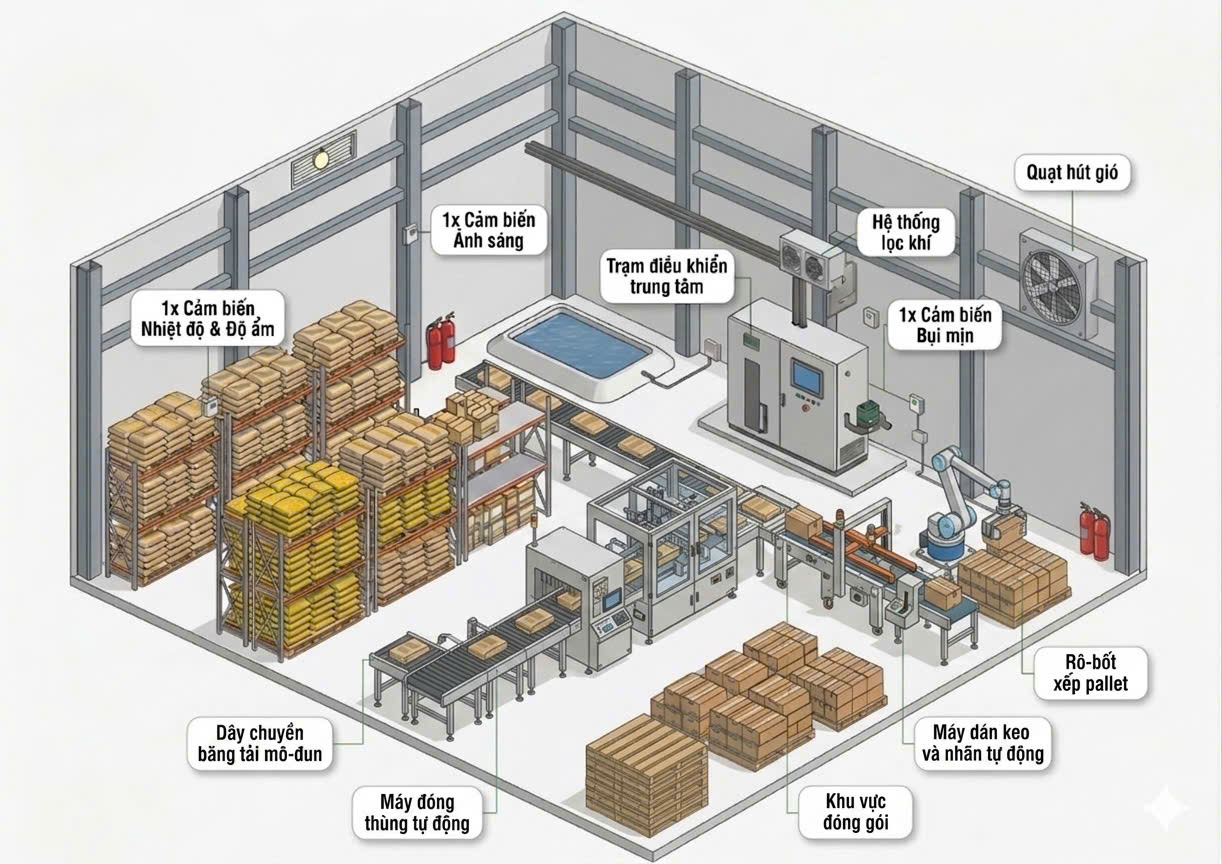
\includegraphics[width=0.5\linewidth]{image/baitoan.jpg}
    \caption{Mô tả bài toán}
    \label{fig:placeholder}
\end{figure}
\subsection{Yêu cầu hệ thống}
\subsubsection{Yêu cầu chức năng}
\begin{table}[H]
\centering
\caption{Yêu cầu chức năng của hệ thống}
\label{tab:functional_requirements}

\begin{tabular}{|c|p{3.5cm}|p{8cm}|}
\hline
\textbf{Mã} & \textbf{Chức năng} & \textbf{Yêu cầu} \\ \hline

FR-01 &
Thu thập dữ liệu &
Hệ thống phải thu thập dữ liệu cảm biến nhiệt độ, độ ẩm, PM2.5 và ánh sáng với chu kỳ tối đa 5 giây/lần. \\ \hline

FR-02 &
Quản lý driver &
Hệ thống phải hỗ trợ giao tiếp I2C và RS485 thông qua driver Linux nhúng. \\ \hline

FR-03 &
Tiền xử lý dữ liệu &
Dữ liệu cảm biến phải được chuẩn hóa và kiểm tra ngưỡng trước khi xử lý. \\ \hline

FR-04 &
Edge Computing &
Gateway phải xử lý dữ liệu và đưa ra quyết định cục bộ với thời gian phản hồi dưới 2 giây. \\ \hline

FR-05 &
Phân tích cảnh báo &
Hệ thống phải phân loại trạng thái thành NORMAL, WARNING, CRITICAL và EMERGENCY\_FIRE. \\ \hline

FR-06 &
Điều khiển thiết bị &
Hệ thống phải hỗ trợ điều khiển relay và quạt làm mát từ Dashboard hoặc Rule Chain. \\ \hline

FR-07 &
Giám sát hệ thống &
Dashboard phải cập nhật telemetry và trạng thái thiết bị theo thời gian thực dưới 5 giây. \\ \hline

FR-08 &
Bảo mật hệ thống &
Hệ thống phải triển khai SELinux, dm-verity và xác thực package trên Yocto Linux. \\ \hline

FR-09 &
Build và custom Yocto &
Hệ thống phải hỗ trợ tự động build và custom image Yocto Linux. \\ \hline

\end{tabular}
\end{table}

\subsubsection{Yêu cầu phi chức năng}
\begin{table}[H]
\centering
\caption{Yêu cầu phi chức năng của hệ thống}
\label{tab:nonfunctional_requirements}

\begin{tabular}{|c|p{3.5cm}|p{8cm}|}
\hline
\textbf{Mã} & \textbf{Yêu cầu} & \textbf{Mô tả} \\ \hline

NFR-01 &
Bảo mật &
Dữ liệu MQTT phải được mã hóa bằng SSL/TLS và hệ thống phải giới hạn truy cập trái phép. \\ \hline

NFR-02 &
Hiệu năng &
Hệ thống phải xử lý và gửi telemetry với độ trễ nhỏ hơn 5 giây. \\ \hline

NFR-03 &
Độ ổn định &
Gateway phải hoạt động liên tục tối thiểu 24 giờ mà không bị treo hoặc mất dữ liệu. \\ \hline

NFR-04 &
Khả năng mở rộng &
Hệ thống phải hỗ trợ mở rộng tối thiểu 10 node IoT hoạt động đồng thời. \\ \hline

NFR-05 &
Tính module &
Driver, Rule Chain và các service phải hoạt động độc lập và dễ dàng mở rộng. \\ \hline

NFR-06 &
Độ tin cậy &
Hệ thống phải duy trì kết nối ổn định với MQTT Broker trong môi trường công nghiệp. \\ \hline

\end{tabular}
\end{table}

\section{Kiến trúc tổng quan hệ thống}

\section{Thiết kế phần cứng hệ thống}
\subsection{Raspberry Pi4}

Trong phạm vi đề tài, Raspberry Pi 4 Model B phiên bản 8GB được lựa chọn làm nền tảng phần cứng trung tâm cho hệ thống Linux Embedded. Việc lựa chọn này dựa trên nhiều yếu tố liên quan đến hiệu năng xử lý, khả năng mở rộng phần cứng, mức độ hỗ trợ hệ điều hành và tính phù hợp đối với các ứng dụng IoT công nghiệp.

Trước hết, Raspberry Pi 4 được trang bị bộ vi xử lý Broadcom BCM2711 kiến trúc ARM Cortex-A72 64-bit với 4 nhân xử lý, cho phép đáp ứng đồng thời nhiều tác vụ như xử lý driver kernel, truyền dữ liệu MQTT, hiển thị giao diện dashboard và thực thi mô-đun AI phân tích dữ liệu. Phiên bản RAM 8GB cũng cung cấp dung lượng bộ nhớ đủ lớn để triển khai các thành phần AI và các dịch vụ Linux Embedded mà không gây thiếu hụt tài nguyên hệ thống.

Các nền tảng vi điều khiển khác như Arduino hoặc ESP32 có ưu điểm về chi phí thấp, mức tiêu thụ năng lượng nhỏ và dễ triển khai đối với các ứng dụng điều khiển đơn giản. Tuy nhiên, các nền tảng này không hỗ trợ đầy đủ hệ điều hành Linux, khả năng đa nhiệm còn hạn chế và khó đáp ứng các yêu cầu xử lý phức tạp như giao tiếp mạng, triển khai AI hoặc tích hợp đồng thời nhiều dịch vụ hệ thống. Do đó, nhóm vi điều khiển này chưa phù hợp với mục tiêu xây dựng một nền tảng Linux Embedded hoàn chỉnh trong đề tài.

Bên cạnh đó, một số bo mạch nhúng hỗ trợ Linux như BeagleBone Black, ODROID-C4 hoặc NanoPi NEO2 cũng được xem xét trong quá trình lựa chọn phần cứng. Mặc dù các nền tảng này hỗ trợ nhiều giao tiếp ngoại vi và có khả năng chạy Yocto Project, tuy nhiên hiệu năng xử lý, dung lượng bộ nhớ và hệ sinh thái phát triển vẫn còn những hạn chế nhất định. Ngoài ra, mức độ phổ biến của các nền tảng này không cao bằng Raspberry Pi, dẫn đến việc thiếu tài liệu kỹ thuật, cộng đồng hỗ trợ và các package phần mềm tối ưu cho Linux Embedded.

Sau quá trình đánh giá, Raspberry Pi 4 Model B được lựa chọn làm nền tảng trung tâm của hệ thống nhờ khả năng cân bằng giữa hiệu năng xử lý, tài nguyên phần cứng, khả năng hỗ trợ Yocto Project và mức độ hoàn thiện của hệ sinh thái phần mềm. 

\begin{table}[H]
\centering 
\caption{So sánh các nền tảng phần cứng hỗ trợ Yocto Project}
\renewcommand{\arraystretch}{1.4}
\begin{tabularx}{\textwidth}{|l|c|c|c|>{\raggedright\arraybackslash}X|}
\hline
\textbf{Board} & \textbf{Yocto} & \textbf{CPU} & \textbf{RAM} & \textbf{Đánh giá tổng quan} \\
\hline
Raspberry Pi 4 & Tốt & A72 & 2--8 GB & Hỗ trợ Yocto ổn định, cộng đồng lớn, nhiều giao tiếp ngoại vi, phù hợp cho Linux Embedded và AIoT \\
\hline
BeagleBone Black & Khá & A8 & 512 MB & Hỗ trợ giao tiếp công nghiệp tốt nhưng hạn chế về hiệu năng và dung lượng RAM \\
\hline
ODROID-C4 & Khá & A55 & 4 GB & Hiệu năng CPU tốt, hỗ trợ Yocto nhưng hệ sinh thái và tài liệu chưa phong phú \\
\hline
NanoPi NEO2 & Trung bình & A53 & 512 MB--1 GB & Chi phí thấp, kích thước nhỏ gọn nhưng hạn chế khả năng mở rộng hệ thống \\
\hline
\end{tabularx}
\end{table}

Từ các kết quả đánh giá và so sánh, có thể thấy Raspberry Pi 4 Model B đáp ứng tốt các yêu cầu của hệ thống Linux Embedded trong đề tài, bao gồm khả năng xử lý đa nhiệm, hỗ trợ giao tiếp phần cứng, tích hợp AIoT và khả năng tùy biến thông qua Yocto Project.

\subsection{Chuẩn giao tiếp vật lý RS485}

Trong các hệ thống nhúng và tự động hóa công nghiệp, việc lựa chọn chuẩn truyền thông đóng vai trò quan trọng đối với độ ổn định và khả năng mở rộng của hệ thống. Trong phạm vi đề tài, chuẩn truyền thông RS485 được lựa chọn để kết nối giữa Raspberry Pi 4 và cảm biến môi trường thay vì các chuẩn truyền thông nối tiếp khác như RS232 hoặc RS422.

Chuẩn RS232 có ưu điểm là đơn giản và dễ triển khai, tuy nhiên khoảng cách truyền ngắn, khả năng chống nhiễu thấp và chỉ hỗ trợ giao tiếp point-to-point. Điều này khiến RS232 không phù hợp với môi trường công nghiệp, nơi thường tồn tại nhiễu điện từ và yêu cầu truyền dữ liệu trên khoảng cách lớn.

Trong khi đó, RS422 hỗ trợ truyền xa và chống nhiễu tốt hơn RS232 nhờ cơ chế truyền vi sai. Tuy nhiên, chuẩn này chủ yếu hỗ trợ giao tiếp một chiều giữa một master và nhiều slave, đồng thời khả năng giao tiếp đa điểm còn hạn chế.

\begin{figure}[H]
    \centering
    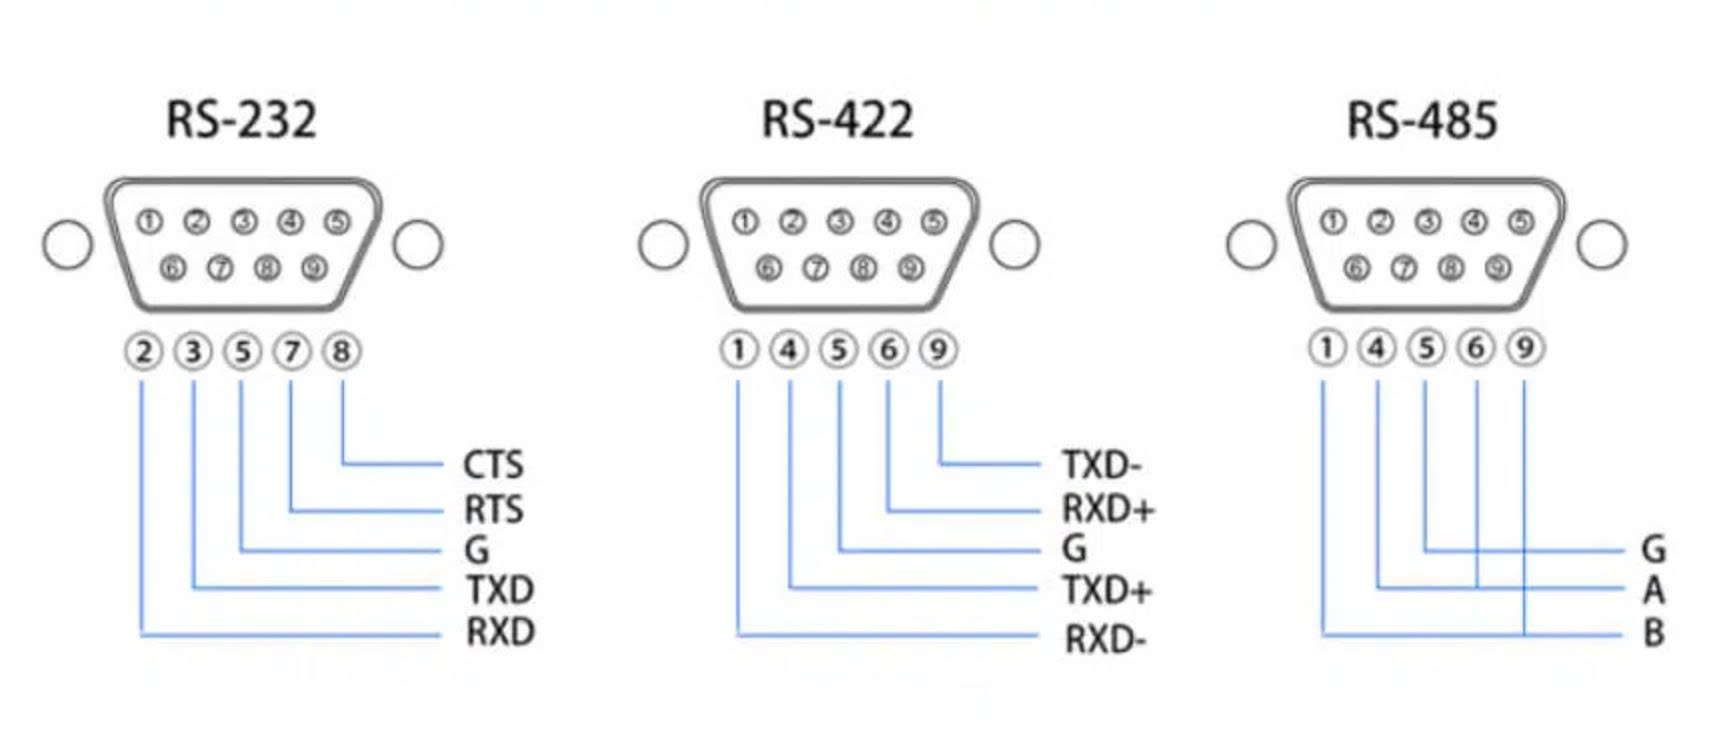
\includegraphics[width=0.75\linewidth]{image/rs.png}
    \caption{Các chuẩn giao tiếp vật lý công nghiệp}
    \label{fig:rs}
\end{figure}

So với các chuẩn trên, RS485 hỗ trợ cơ chế truyền vi sai giúp tăng khả năng chống nhiễu và đảm bảo độ ổn định trong môi trường công nghiệp. Chuẩn này cho phép nhiều thiết bị cùng kết nối trên một bus truyền thông, hỗ trợ khoảng cách truyền lớn và có khả năng hoạt động ổn định trong điều kiện nhiễu điện từ cao. Ngoài ra, RS485 cũng được sử dụng phổ biến trong các giao thức công nghiệp như Modbus RTU, giúp thuận lợi cho việc tích hợp cảm biến và mở rộng hệ thống trong tương lai.

Bên cạnh đó, RS485 có cấu trúc phần cứng tương đối đơn giản, dễ tích hợp với UART của Raspberry Pi thông qua IC chuyển đổi MAX485. Điều này giúp giảm chi phí triển khai nhưng vẫn đảm bảo hiệu quả truyền nhận dữ liệu trong hệ thống Linux Embedded.

Từ các đặc điểm trên, RS485 được đánh giá là phù hợp hơn cho bài toán giám sát môi trường công nghiệp của đề tài, đặc biệt trong các yêu cầu về độ ổn định, khả năng chống nhiễu và hỗ trợ mở rộng hệ thống IoT.

\section{Thiết kế nền tảng nhúng}
\subsection{Thiết kế hệ thống bảo mật cho Linux nhúng}
\subsubsection{Xây dựng cơ chế kiểm soát truy cập và phân quyền}
Hệ thống thiết kế cơ chế phân quyền người dùng bằng \texttt{sudo} nhằm giới hạn phạm vi thao tác trên thiết bị Yocto Linux. Tài khoản \texttt{gatewayadmin} được cấp quyền thực thi và quản lý các ứng dụng cần thiết của hệ thống, tuy nhiên không được phép thực hiện các thao tác ảnh hưởng đến toàn bộ hệ thống như chỉnh sửa file hệ thống, reboot thiết bị hoặc thay đổi cấu hình bảo mật.

Các quyền được cấu hình thông qua file \texttt{/etc/sudoers.d/} nhằm kiểm soát chính xác các lệnh mà người dùng được phép thực thi. Cơ chế này giúp tăng cường bảo mật và hạn chế các thao tác trái phép trên hệ thống Linux nhúng.

\subsubsection{Tăng cường bảo mật dịch vụ SSH}
\begin{figure}[H]
    \centering
    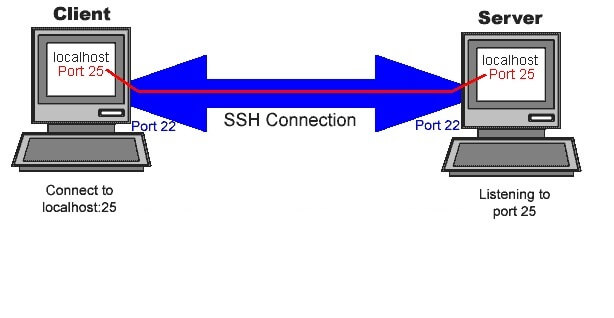
\includegraphics[width=0.4\textwidth]{image/ssh.jpg}
    \caption{Cơ chế SSH}
    \label{fig:ssh}
\end{figure}

SSH (Secure Shell) là giao thức được sử dụng để truy cập và quản trị hệ thống Linux từ xa. Trong các hệ thống Linux nhúng xây dựng bằng Yocto Linux, SSH đóng vai trò quan trọng trong quá trình cấu hình, giám sát và bảo trì thiết bị. Tuy nhiên, dịch vụ SSH cũng là một trong những mục tiêu tấn công phổ biến do thường được mở trên môi trường mạng.

Để nâng cao mức độ an toàn cho thiết bị, Nhóm tiến hành thiết kế cơ chế SSH Hardening nhằm tăng cường khả năng bảo mật và kiểm soát truy cập đối với dịch vụ SSH. Kiến trúc tổng quan của cơ chế bảo mật SSH được thể hiện trong Hình \ref{fig:ssh_hardening}.

\begin{figure}[H]
    \centering
    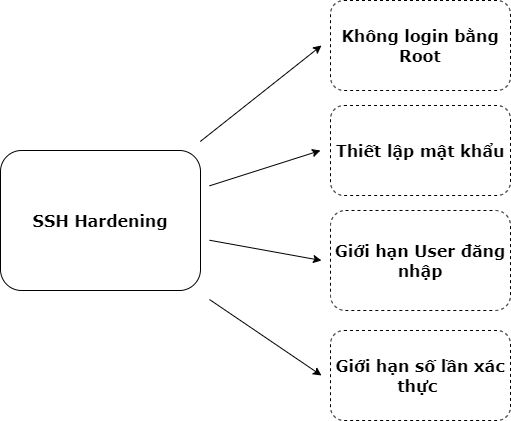
\includegraphics[width=0.5\textwidth]{image/ssh_tk.png}
    \caption{Thiết kế cơ chế tăng cường bảo mật SSH}
    \label{fig:ssh_hardening}
\end{figure}

Nhóm thiết lập cơ chế SSH Hardening được thiết kế bao gồm các chức năng chính như sau:

Thứ nhất, nhóm thiết kế vô hiệu hóa chức năng đăng nhập trực tiếp bằng tài khoản \texttt{root} thông qua giao thức SSH. Người dùng không được phép truy cập trực tiếp với quyền quản trị cao nhất mà phải đăng nhập bằng tài khoản thông thường trước khi sử dụng cơ chế nâng quyền. Điều này giúp hạn chế nguy cơ tấn công trực tiếp vào tài khoản quản trị hệ thống và giảm thiểu khả năng khai thác trái phép từ bên ngoài mạng.

Thứ hai, nhóm thiết kế cơ chế thiết lập chính sách mật khẩu nhằm tăng cường mức độ an toàn cho tài khoản người dùng khi đăng nhập SSH. Chính sách mật khẩu được thiết kế với các yêu cầu về độ dài tối thiểu, mức độ phức tạp và thời gian sử dụng mật khẩu. Các quy tắc mật khẩu được tích hợp thông qua PAM (Pluggable Authentication Modules) trên Yocto Linux nhằm đảm bảo tính linh hoạt và khả năng quản lý tập trung trong hệ thống.

Thứ ba, nhóm thiết kế cơ chế kiểm soát danh sách người dùng được phép truy cập SSH. Chỉ các tài khoản nằm trong danh sách cho phép mới có quyền đăng nhập từ xa vào thiết bị. Cơ chế này giúp kiểm soát quyền truy cập, hạn chế việc sử dụng các tài khoản không hợp lệ và giảm bề mặt tấn công của hệ thống.

Thứ tư, để tăng cường khả năng chống lại các cuộc tấn công brute-force, hệ thống thiết kế cơ chế giới hạn số lần xác thực đăng nhập SSH. Khi số lần nhập sai vượt quá ngưỡng cho phép, kết nối đăng nhập sẽ bị từ chối hoặc tạm thời khóa trong một khoảng thời gian nhất định. Ngoài ra, hệ thống cũng thiết lập thời gian giới hạn cho quá trình xác thực nhằm tránh việc duy trì kết nối SSH không cần thiết trong thời gian dài.

\subsubsection{Thiết kế hệ thống quản lý package an toàn}

Trong các hệ thống Linux nhúng sử dụng Yocto Linux, cơ chế quản lý package đóng vai trò quan trọng trong việc cập nhật chức năng, bảo trì và mở rộng hệ thống. Tuy nhiên, nếu không có cơ chế kiểm soát phù hợp, người dùng có thể cài đặt các package không đáng tin cậy hoặc package đã bị thay đổi nội dung, từ đó ảnh hưởng đến tính toàn vẹn và mức độ an toàn của thiết bị.

Trong luận văn này, nhóm thực hiện đề xuất kiến trúc quản lý package theo hướng kiểm soát tập trung nhằm tăng cường khả năng xác thực và kiểm soát quá trình cài đặt package trên thiết bị nhúng. Hệ thống được thiết kế để mọi package trước khi cài đặt đều phải trải qua các bước kiểm tra bảo mật và xác thực nguồn gốc.

\vspace{0.5em}

\noindent\textbf{Lựa chọn package manager cho hệ thống} \\

Trên các hệ thống Linux nhúng hiện nay, một số package manager phổ biến bao gồm DPKG, RPM và OPKG. Mỗi cơ chế quản lý package có đặc điểm riêng về kiến trúc, hiệu năng và mức độ phù hợp đối với các hệ thống nhúng có tài nguyên hạn chế. Trong quá trình nghiên cứu và thiết kế hệ thống, nhóm đã tiến hành đánh giá các package manager phổ biến nhằm lựa chọn giải pháp phù hợp cho nền tảng Yocto Linux được sử dụng trong luận văn.

Bảng \ref{tab:package_manager_compare} trình bày so sánh giữa DPKG, RPM và OPKG trong môi trường Linux nhúng.
\begin{table}[H]
\centering
\caption{So sánh các package manager trên Linux}
\label{tab:package_manager_compare}

\begin{tabular}{|l|c|c|c|}
\hline
\textbf{Tiêu chí} & \textbf{DPKG} & \textbf{RPM} & \textbf{OPKG} \\ \hline

Định dạng package &
\texttt{.deb} &
\texttt{.rpm} &
\texttt{.ipk} \\ \hline

Dung lượng hệ thống &
Trung bình &
Lớn &
Nhẹ \\ \hline

Hiệu năng Embedded &
Trung bình &
Trung bình &
Tốt \\ \hline

Quản lý dependency &
Đầy đủ &
Đầy đủ &
Đơn giản \\ \hline

Mức phù hợp Embedded &
Khá phù hợp &
Hệ thống lớn &
Rất phù hợp \\ \hline

Hệ thống phổ biến &
Ubuntu &
Fedora &
Yocto \\ \hline

\end{tabular}
\end{table}

Từ kết quả đánh giá, nhóm lựa chọn OPKG làm package manager chính cho hệ thống do có kiến trúc gọn nhẹ, khả năng xử lý nhanh và phù hợp với các thiết bị Linux nhúng có tài nguyên phần cứng hạn chế như Raspberry Pi 4.

\noindent\textbf{Thiết kế repository quản lý package}

\begin{figure}[H]
    \centering
    
\includegraphics[width=0.5\textwidth]{image/nginx.jpg}
    \caption{Nginx repository server cho quản lý package an toàn}
    \label{fig:nginx}
\end{figure}

Trong kiến trúc được đề xuất, nhóm sử dụng Nginx như một repository server nội bộ để lưu trữ và phân phối package đến thiết bị nhúng. Nginx là web server có hiệu năng cao, khả năng xử lý nhẹ và phù hợp cho việc cung cấp các tệp tĩnh thông qua giao thức HTTP. Repository của hệ thống bao gồm các package \texttt{.ipk}, file metadata \texttt{Packages.gz}, chữ ký số \texttt{Packages.gz.asc} và khóa công khai \texttt{public.key}.


\noindent\textbf{Tổng quan thiết kế hệ thống quản lý package an toàn}

Trong luận văn này, nhóm đề xuất cơ chế cài đặt package thông qua lớp trung gian thay vì cho phép người dùng truy cập trực tiếp package manager của hệ thống. Kiến trúc tổng quan của cơ chế quản lý package được mô tả như sau:

\begin{figure}[H]
    \centering
    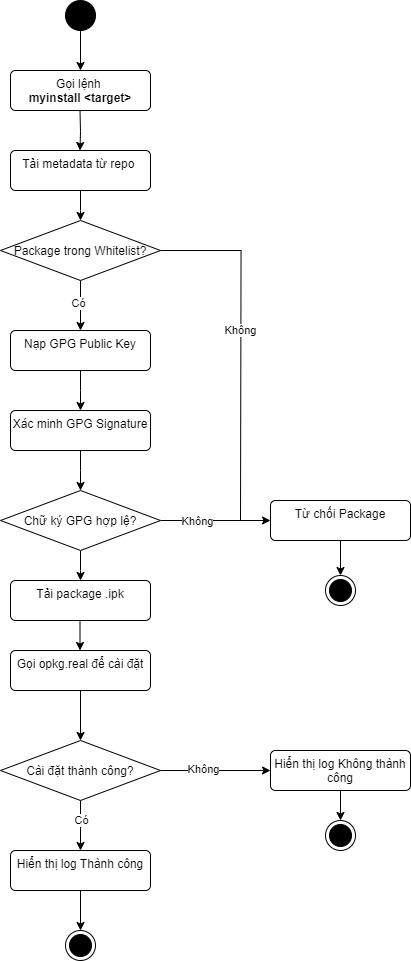
\includegraphics[width=0.4\textwidth]{image/pack_diagram.jpg}
    \caption{Kiến trúc quản lý package an toàn}
    \label{fig:pack_diagram}
\end{figure}

Trong kiến trúc này, lớp trung gian \texttt{myinstall} được nhóm thiết kế nhằm thực hiện các bước xác thực package trước khi cho phép cài đặt thực tế trên hệ thống. Cách tiếp cận này giúp tăng cường khả năng kiểm soát package và hạn chế nguy cơ cài đặt package trái phép hoặc package không đáng tin cậy.

\vspace{0.5em}


Để kiểm soát danh sách package được phép cài đặt, nhóm đề xuất cơ chế whitelist nhằm giới hạn các package hợp lệ trên hệ thống. Theo thiết kế, chỉ các package tồn tại trong danh sách cho phép mới được tiếp tục quá trình xác thực và cài đặt. Điều này giúp giảm bề mặt tấn công và hạn chế nguy cơ cài đặt các package không thuộc phạm vi quản lý của hệ thống.

Bên cạnh cơ chế whitelist, nhóm cũng thiết kế cơ chế xác thực chữ ký số GPG nhằm đảm bảo tính toàn vẹn của repository package. Ở đây, metadata repository sẽ được ký bằng khóa bí mật trên máy host và được xác thực bằng khóa công khai trên thiết bị nhúng trước khi cho phép cài đặt package. Điều này giúp hệ thống phát hiện các trường hợp package hoặc metadata bị thay đổi nội dung trong quá trình truyền tải, từ đó hạn chế nguy cơ giả mạo repository hoặc tấn công chèn mã độc vào package.

Trong hệ thống được đề xuất, nhóm không cho phép người dùng sử dụng trực tiếp package manager mặc định của hệ thống. Thay vào đó, mọi thao tác cài đặt package phải đi qua lớp kiểm soát trung gian do nhóm xây dựng. Điều này giúp đảm bảo toàn bộ quá trình cài đặt luôn tuân theo chính sách xác thực và kiểm tra bảo mật đã được thiết kế trong hệ thống. Ngoài ra, backend package manager thực tế cũng được nhóm giới hạn quyền truy cập nhằm giảm nguy cơ khai thác trái phép hoặc bỏ qua cơ chế kiểm soát bảo mật của hệ thống.

\subsubsection{Triển khai cơ chế bảo mật SELinux}

SELinux (Security-Enhanced Linux) là cơ chế bảo mật dành cho Linux dựa trên mô hình Mandatory Access Control (MAC), cho phép kiểm soát quyền truy cập giữa tiến trình và tài nguyên hệ thống thông qua các policy bảo mật. Trong hệ thống Yocto Linux, SELinux được tích hợp thông qua layer \texttt{meta-selinux} nhằm tăng cường khả năng bảo vệ cho hệ điều hành nhúng.

Trong quá trình thiết kế hệ thống, đề tài sử dụng SELinux nhằm giới hạn quyền truy cập của tiến trình và giảm thiểu ảnh hưởng khi dịch vụ bị khai thác. SELinux hoạt động dựa trên security context và các policy được định nghĩa sẵn, theo nguyên tắc mặc định từ chối truy cập nếu không được cho phép rõ ràng.

\begin{figure}[!h]
    \centering
    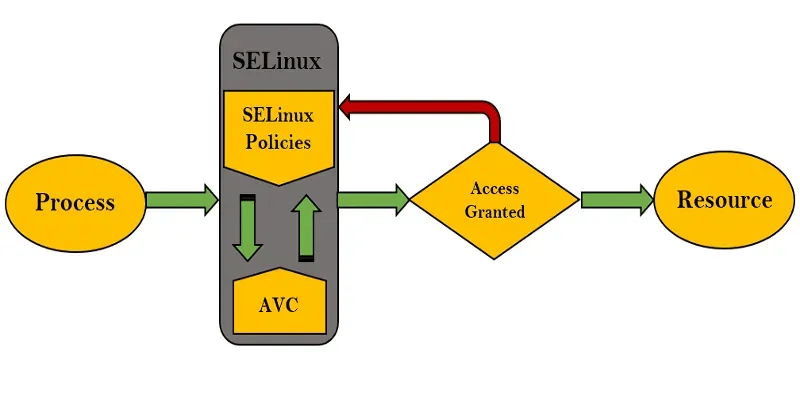
\includegraphics[width=0.7\textwidth]{image/image3.png}
    \caption{Bảo mật quyền truy cập hệ thống với SELinux trong Yocto}
    \label{fig:selinux}
\end{figure}

SELinux cung cấp nhiều loại policy khác nhau phục vụ cho từng mục đích triển khai hệ thống. Bảng \ref{tab:selinux_policy} trình bày một số policy phổ biến của SELinux.

\begin{table}[H]
\centering
\caption{So sánh các policy trong SELinux}
\label{tab:selinux_policy}
\begin{tabular}{|p{3cm}|p{4cm}|p{5cm}|}
\hline
\textbf{Policy} & \textbf{Đặc điểm} & \textbf{Mục đích sử dụng} \\ \hline

\texttt{targeted} & Chỉ bảo vệ các dịch vụ và tiến trình quan trọng & Phù hợp cho hệ thống thực tế, dễ triển khai và tương thích cao \\ \hline

\texttt{minimum} & Chỉ chứa các policy tối thiểu cần thiết & Dùng cho hệ thống nhúng hoặc hệ thống yêu cầu tối giản \\ \hline

\texttt{mls} & Hỗ trợ Multi-Level Security với nhiều mức bảo mật & Sử dụng trong hệ thống yêu cầu bảo mật nghiêm ngặt \\ \hline

\end{tabular}
\end{table}

Trong đề tài này, hệ thống lựa chọn policy \texttt{targeted} do đây là policy phổ biến và phù hợp với môi trường Linux nhúng trên Yocto. Policy này tập trung bảo vệ các dịch vụ quan trọng như SSH, systemd hoặc web server, đồng thời vẫn đảm bảo khả năng tương thích và dễ triển khai trên thiết bị nhúng.

SELinux được cấu hình ở chế độ enforcing nhằm đảm bảo mọi truy cập không hợp lệ sẽ bị từ chối theo policy đã định nghĩa trước. Việc sử dụng policy mặc định giúp giảm độ phức tạp trong quá trình phát triển hệ thống, đồng thời vẫn đảm bảo tăng cường bảo mật cho thiết bị Yocto Linux.
\subsubsection{Bảo vệ tính toàn vẹn hệ thống với dm-verity}

Trong các hệ thống Linux nhúng, việc bảo vệ tính toàn vẹn của phân vùng hệ thống tập tin gốc (root filesystem) là một yêu cầu quan trọng nhằm ngăn chặn các hành vi chỉnh sửa trái phép trên thiết bị lưu trữ. Đặc biệt, trong các kịch bản tấn công offline, kẻ tấn công có thể can thiệp trực tiếp vào thẻ nhớ hoặc bộ nhớ ngoài để thay đổi dữ liệu hệ thống mà không cần truy cập vào hệ điều hành đang chạy. Để giải quyết vấn đề này, trong luận văn nhóm đã nghiên cứu và hiện thực cơ chế \texttt{dm-verity} trên nền tảng Linux nhúng.

\texttt{dm-verity} (Device Mapper Verity) là một cơ chế xác thực dữ liệu ở mức khối, được tích hợp trong Linux kernel thông qua Device Mapper. Cơ chế này sử dụng cấu trúc cây băm Merkle (Merkle Hash Tree) để kiểm tra tính toàn vẹn của từng block dữ liệu trong phân vùng rootfs. Mỗi block dữ liệu được băm để tạo ra các giá trị hash ở các cấp thấp hơn; các giá trị này tiếp tục được băm lên nhiều cấp cho đến khi thu được một hash gốc duy nhất. Hash gốc này đại diện cho toàn bộ nội dung của hệ thống tập tin và được sử dụng làm cơ sở để xác minh dữ liệu trong quá trình khởi động và truy cập hệ thống.

Hình~\ref{fig:merkle_hash_tree} minh họa cấu trúc cây Merkle Hash Tree mà nhóm đã sử dụng trong quá trình nghiên cứu và hiện thực cơ chế xác thực toàn vẹn cho rootfs. Trong mô hình này, khi một block dữ liệu bị thay đổi, giá trị hash tương ứng sẽ không còn khớp với các hash ở cấp cao hơn, từ đó hệ thống có thể phát hiện sớm sự can thiệp trái phép và ngăn chặn việc sử dụng dữ liệu đã bị chỉnh sửa.

\begin{figure}[htbp]
    \centering
    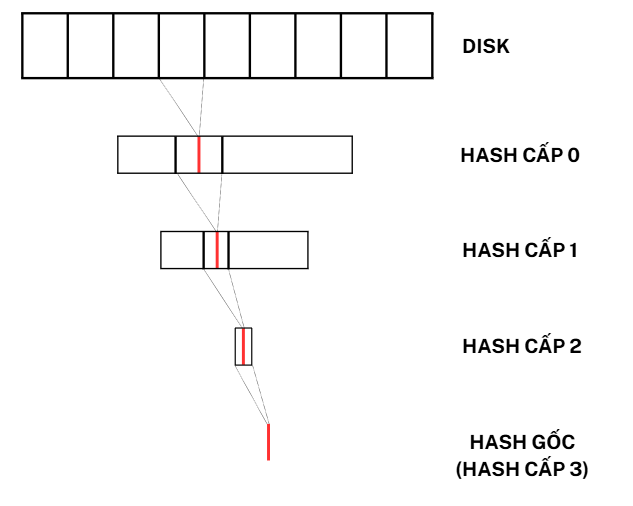
\includegraphics[width=0.4\linewidth]{image/image4.png}
    \caption{Cấu trúc Merkle Hash Tree trong cơ chế dm-verity}
    \label{fig:merkle_hash_tree}
\end{figure}

Trong luận văn, nhóm đã thiết kế hệ thống dm-verity theo hướng kết hợp giữa quá trình tạo ảnh hệ thống và quá trình kiểm tra tính toàn vẹn khi thiết bị khởi động. Kiến trúc tổng thể của hệ thống gồm hai giai đoạn chính: giai đoạn chuẩn bị image trên máy phát triển và giai đoạn xác thực rootfs trên thiết bị đích.

Ở giai đoạn chuẩn bị image, sau khi hoàn tất quá trình build hệ điều hành, nhóm đã tiến hành tách phân vùng rootfs từ file \texttt{.wic} và sử dụng công cụ \texttt{veritysetup} để tạo ra cây hash tương ứng. Từ đó, hệ thống sinh ra hai thành phần quan trọng là \texttt{root.hash} và \texttt{rootfs.hash}. Trong đó, \texttt{rootfs.hash} chứa dữ liệu hash tree phục vụ xác thực các block dữ liệu, còn \texttt{root.hash} là giá trị hash gốc được dùng để xác minh toàn bộ cấu trúc. Sau khi tạo xong, image được flash vào thẻ SD và giá trị hash gốc được tích hợp vào kernel hoặc initramfs nhằm đảm bảo tính tin cậy trong quá trình khởi động.

Ở giai đoạn khởi động thiết bị, kernel và initramfs sẽ khởi tạo cơ chế dm-verity trước khi mount phân vùng rootfs. Hệ thống sẽ sử dụng giá trị hash gốc đã được chuẩn bị từ trước để kiểm tra chuỗi hash của toàn bộ phân vùng. Nếu tất cả các giá trị băm đều khớp, rootfs sẽ được mount bình thường và hệ điều hành tiếp tục khởi động. Ngược lại, nếu phát hiện có sự sai lệch tại bất kỳ cấp hash nào, hệ thống sẽ từ chối mount rootfs và dừng quá trình khởi động nhằm ngăn chặn việc sử dụng dữ liệu không còn đảm bảo tính toàn vẹn.

Hình~\ref{fig:dmverity_activity} mô tả activity diagram của hệ thống mà nhóm đã hiện thực trong luận văn. Sơ đồ cho thấy luồng xử lý bắt đầu từ bước build image, tạo hash tree, flash image vào thẻ SD, sau đó thiết bị khởi động và tiến hành kiểm tra toàn vẹn trước khi mount rootfs. Cách tổ chức này cho phép hệ thống chỉ chấp nhận image hợp lệ, đồng thời tăng cường khả năng chống lại các hình thức tấn công can thiệp offline vào thiết bị lưu trữ.

\begin{figure}[htbp]
    \centering
    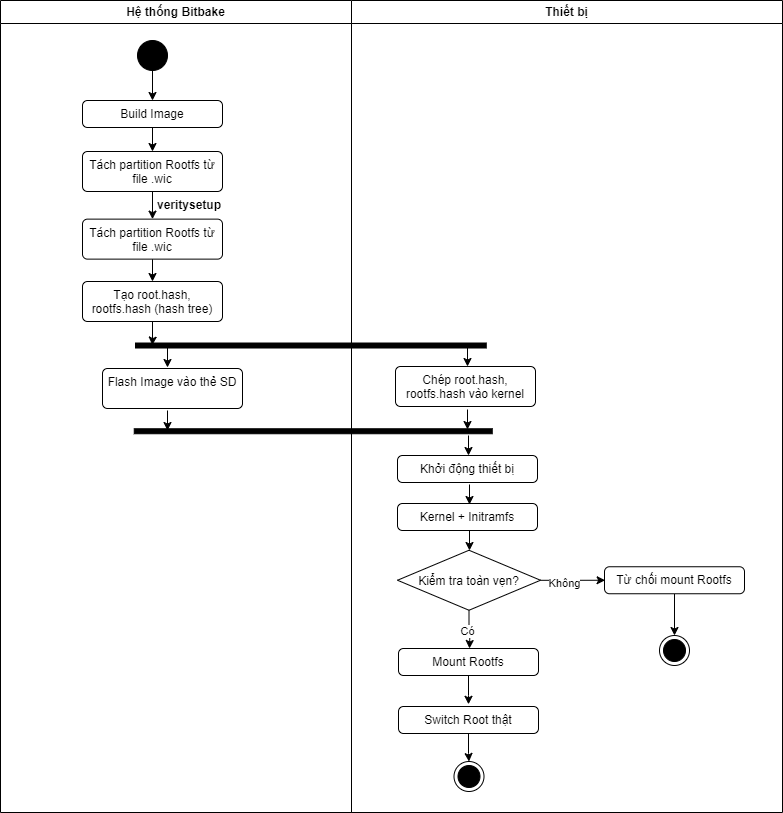
\includegraphics[width=0.6\linewidth]{image/dm.png}
    \caption{Activity diagram thiết kế dm-verity}
    \label{fig:dmverity_activity}
\end{figure}


\subsection{Phát triển Driver cho Linux nhúng}
\subsubsection{Kiến trúc tổng quan Driver trong hệ thống Yocto Linux}

Trong hệ thống Linux nhúng sử dụng Yocto Project, driver đóng vai trò là lớp trung gian giữa tầng ứng dụng và phần cứng ngoại vi. Driver chịu trách nhiệm quản lý giao tiếp phần cứng, cung cấp interface chuẩn cho user space và thực hiện điều khiển thiết bị ở mức thấp thông qua Linux kernel.

Trong đề tài, nhóm không sử dụng các driver giao tiếp mặc định của hệ thống mà tự xây dựng các custom driver cho giao thức I2C và RS485 nhằm tăng tính tùy biến và phù hợp với yêu cầu của hệ thống tự động hóa công nghiệp.

Kiến trúc tổng quan của hệ thống driver được mô tả theo mô hình phân lớp như Hình~\ref{fig:yocto_driver_architecture}.

\begin{figure}[!h]
    \centering
    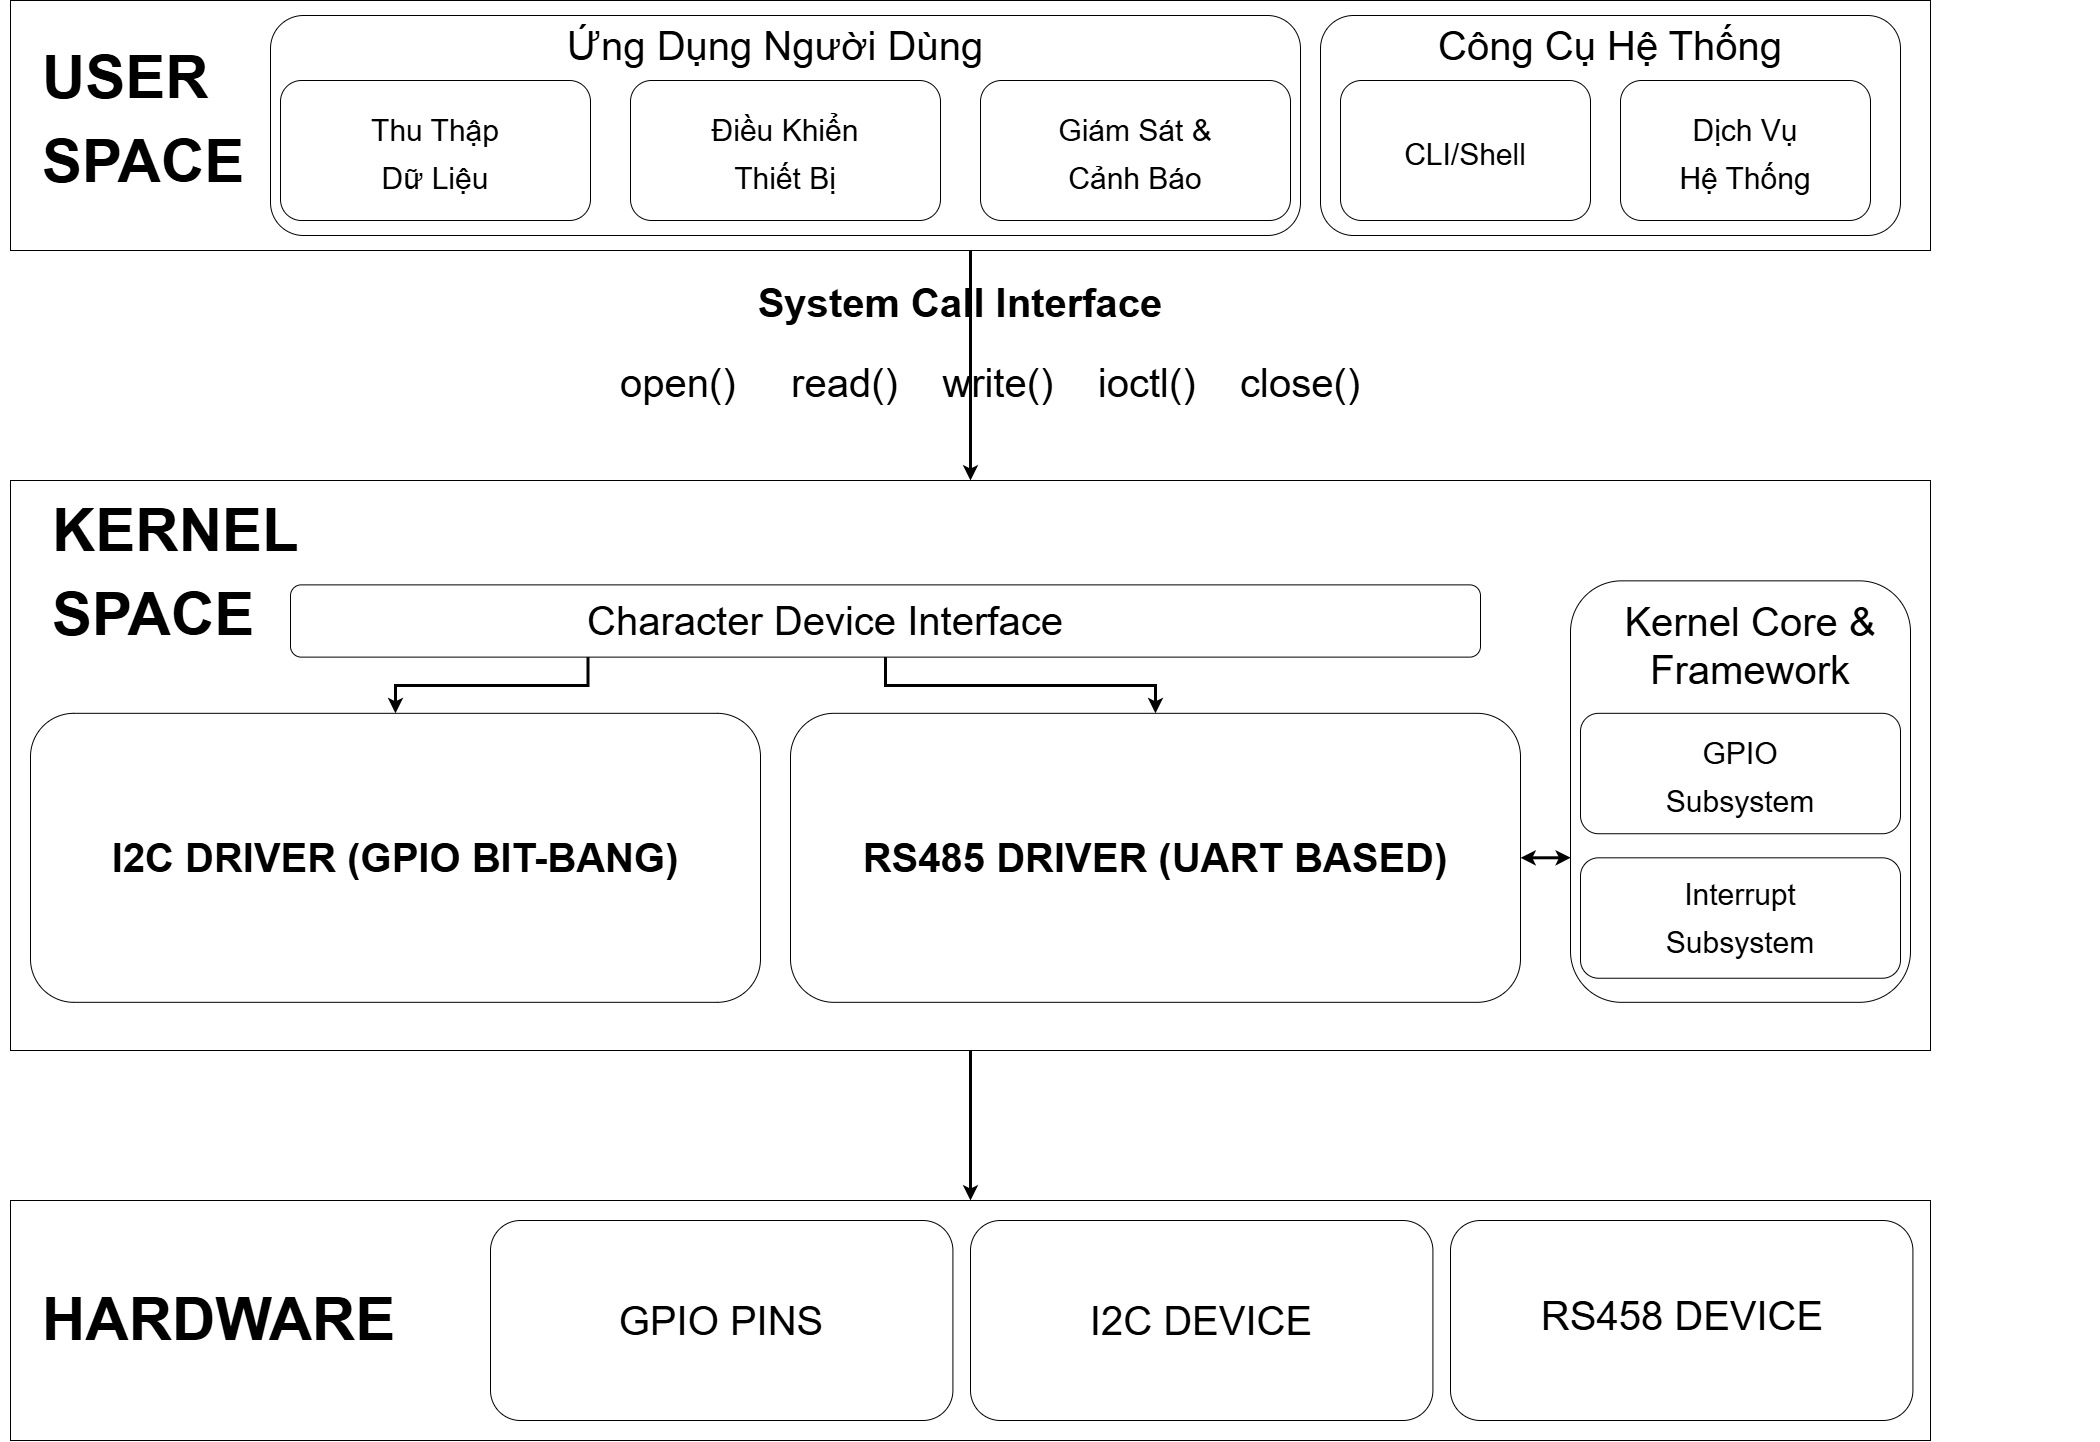
\includegraphics[width=1\textwidth]{image/yocto_driver_architecture.png}
    \caption{Kiến trúc tổng quan driver trong hệ thống Yocto Linux}
    \label{fig:yocto_driver_architecture} 

\end{figure}
\newpage

Trong kiến trúc này, tầng \textbf{User Space} bao gồm các ứng dụng điều khiển, dashboard giám sát và các chương trình xử lý dữ liệu cảm biến. Các ứng dụng này giao tiếp với driver thông qua các system call chuẩn của Linux như \texttt{open()}, \texttt{read()}, \texttt{write()} và \texttt{ioctl()}.

Tầng \textbf{Kernel Space} bao gồm các custom character device driver do nhóm phát triển. Các driver này chịu trách nhiệm xử lý logic giao tiếp, điều khiển GPIO, quản lý timing truyền dữ liệu và tạo các tín hiệu giao tiếp phần cứng.

Driver I2C được hiện thực theo cơ chế software bit-banging nhằm điều khiển trực tiếp hai đường tín hiệu SDA và SCL thông qua GPIO. Driver RS485 được xây dựng để quản lý truyền nhận UART và điều khiển chiều truyền dữ liệu của module RS485 phục vụ giao tiếp Modbus RTU.

Các driver được đóng gói thành kernel module và tích hợp vào hệ thống Yocto thông qua custom layer và BitBake recipe. Sau khi build image, các module driver sẽ được nạp vào Linux kernel và tạo device file trong thư mục \texttt{/dev} để user space có thể truy cập.

Ở tầng thấp nhất, driver giao tiếp trực tiếp với phần cứng ngoại vi như cảm biến, màn hình OLED, relay và các thiết bị công nghiệp sử dụng chuẩn RS485.

Kiến trúc này giúp hệ thống có tính mô-đun cao, dễ mở rộng và phù hợp với các ứng dụng Linux nhúng yêu cầu khả năng tùy biến giao tiếp phần cứng.

\subsubsection{Driver RS485}
\noindent \textbf{Mô hình FSM của driver RS485}

Để quản lý quá trình truyền nhận dữ liệu và xử lý lỗi trong môi trường Linux Kernel, driver được thiết kế theo mô hình máy trạng thái (Finite State Machine – FSM). Mô hình này giúp tổ chức luồng hoạt động của driver một cách rõ ràng, đồng thời hỗ trợ việc kiểm soát các trạng thái truyền nhận và xử lý lỗi trong quá trình giao tiếp RS485 Modbus RTU.

\begin{figure}[!h]
    \centering
    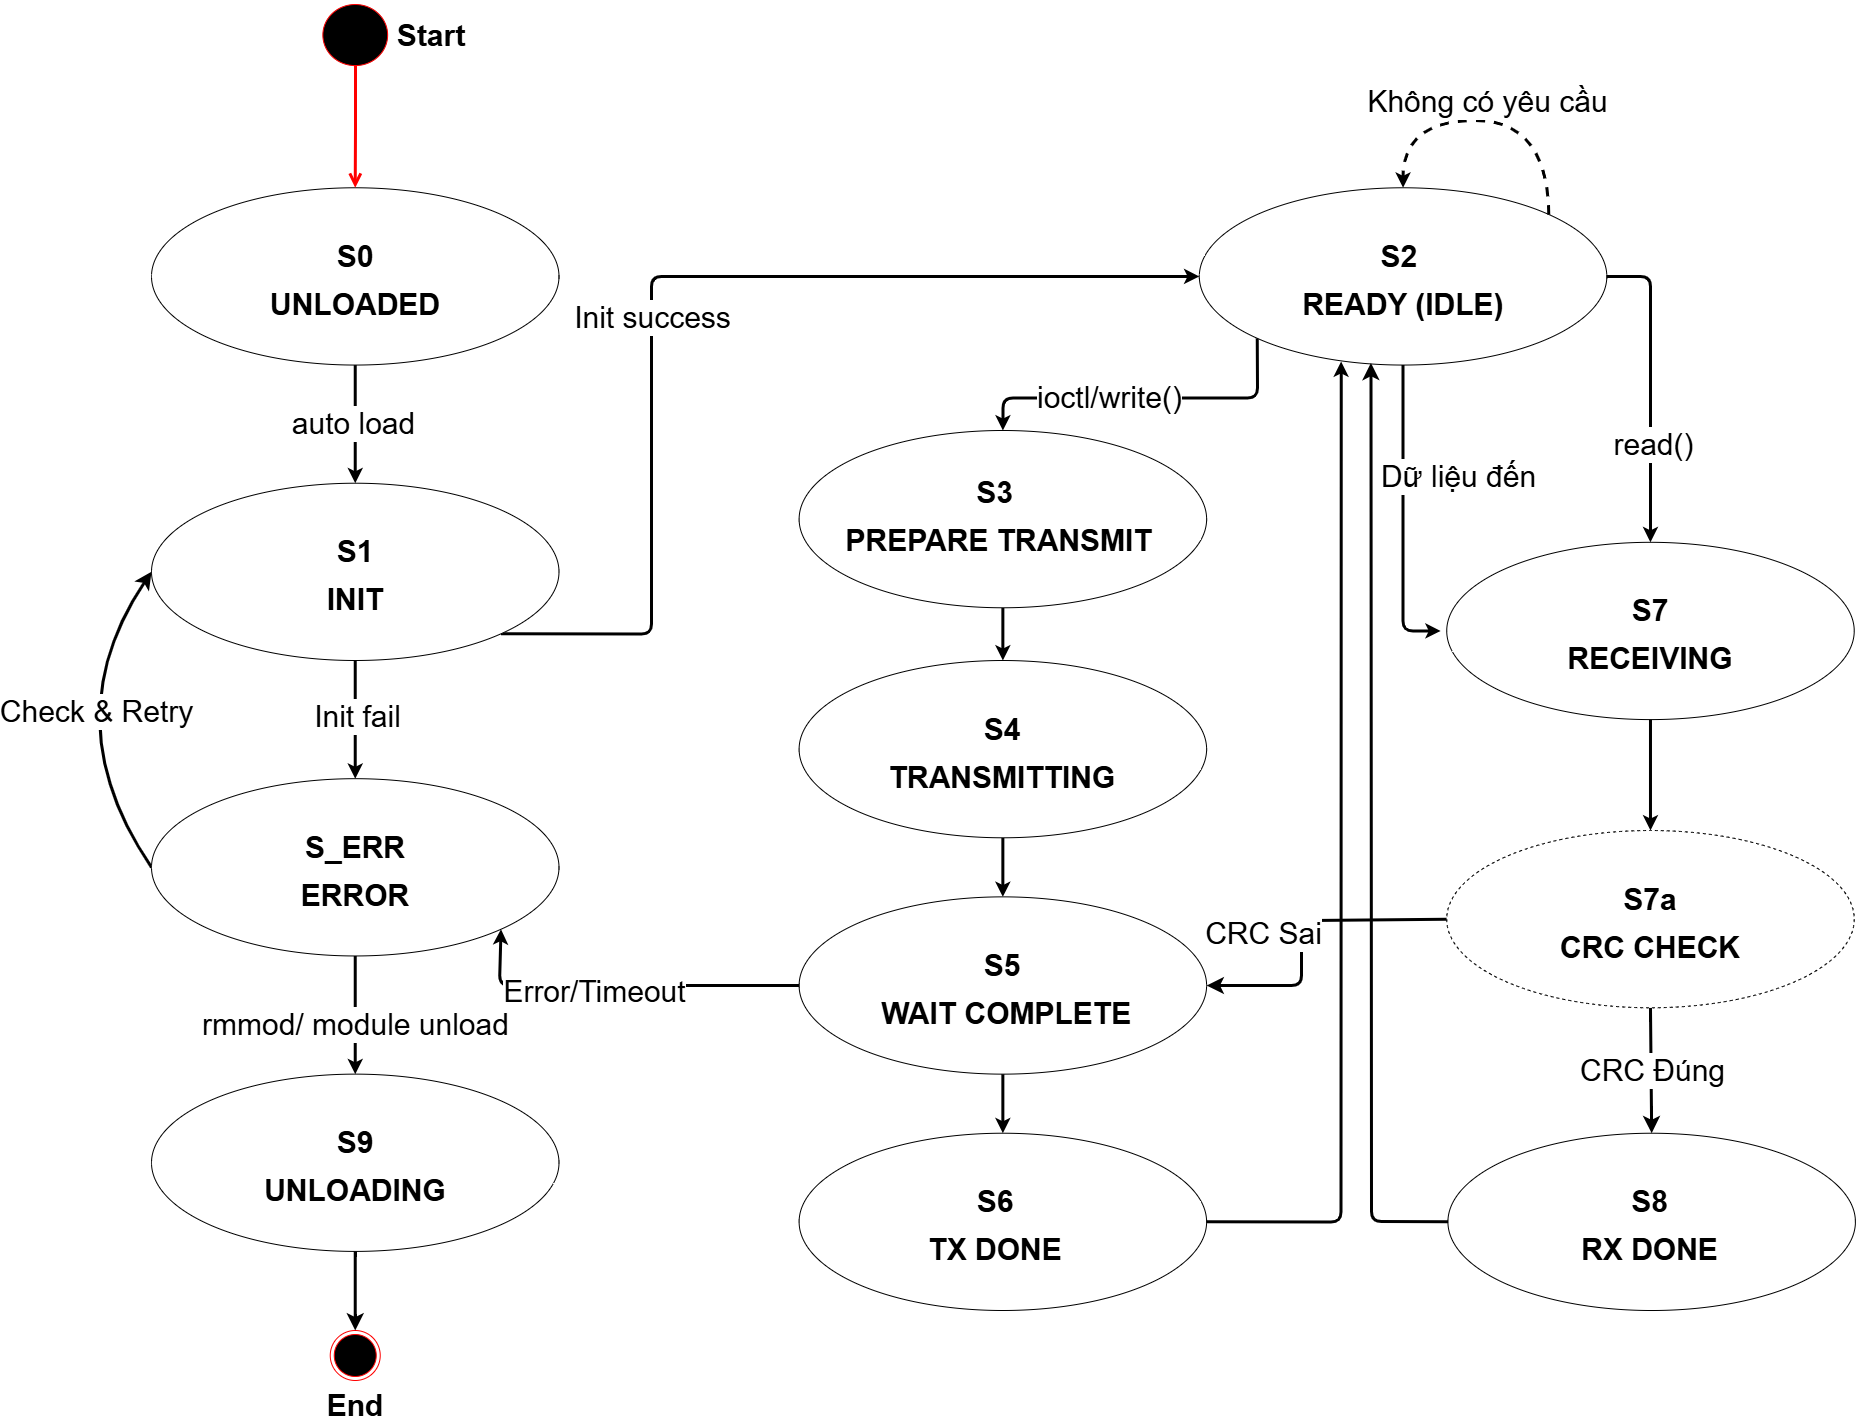
\includegraphics[width=0.8\textwidth]{image/rs485fsm.png}
    \caption{Máy trạng thái cho driver RS458}
    \label{fig:rs485_fsm} 

\end{figure}

FSM của driver RS485 bao gồm các trạng thái chính như mô tả ở Hình \ref{fig:rs485_fsm}. Sau khi hệ thống khởi động, driver bắt đầu tại trạng thái \texttt{UNLOADED}. Khi kernel module được tự động nạp thông qua cơ chế \texttt{autoload}, driver chuyển sang trạng thái \texttt{INIT} để thực hiện khởi tạo UART, GPIO điều khiển DE/RE và các tài nguyên nội bộ của kernel module.

Nếu quá trình khởi tạo thành công, driver chuyển sang trạng thái \texttt{READY (IDLE)} và chờ yêu cầu truyền nhận dữ liệu từ User Space hoặc kernel thread polling. Trong trường hợp khởi tạo thất bại, driver sẽ chuyển sang trạng thái \texttt{ERROR}, đồng thời thực hiện cơ chế retry hoặc chờ unload module khỏi hệ thống.

Khi có yêu cầu đọc hoặc ghi dữ liệu, driver chuyển sang trạng thái \texttt{PREPARE TRANSMIT} để xây dựng khung Modbus RTU và tính toán CRC16 cho gói tin. Sau đó dữ liệu được gửi qua UART trong trạng thái \texttt{TRANSMITTING}. Khi quá trình truyền hoàn tất, driver chuyển sang trạng thái \texttt{WAIT COMPLETE} để chờ phản hồi từ thiết bị slave.

Sau khi nhận được dữ liệu phản hồi, driver thực hiện kiểm tra CRC trong trạng thái \texttt{CRC CHECK}. Nếu CRC hợp lệ, driver tiếp tục chuyển sang trạng thái \texttt{RECEIVING} để giải mã dữ liệu thanh ghi Modbus, sau đó chuyển sang trạng thái \texttt{RX DONE} nhằm cập nhật cache dữ liệu và cung cấp dữ liệu cho User Space. Ngược lại, nếu CRC không hợp lệ hoặc xảy ra timeout trong quá trình truyền nhận, driver sẽ chuyển sang trạng thái \texttt{ERROR} để xử lý lỗi truyền thông.

Cuối cùng, khi kernel module bị gỡ khỏi hệ thống thông qua lệnh \texttt{rmmod}, driver chuyển sang trạng thái \texttt{UNLOADING} để giải phóng tài nguyên và kết thúc vòng đời hoạt động của module trong Linux Kernel.

\noindent \textbf{Activity Diagram của driver RS485}

Trong khi FSM tập trung mô tả các trạng thái nội bộ của driver, quá trình tương tác thực tế giữa User Space, Kernel Space và phần cứng UART được thể hiện thông qua Activity Diagram. Sơ đồ này mô tả tuần tự các bước xử lý khi ứng dụng thực hiện các thao tác đọc, ghi và cấu hình thiết bị thông qua system call trong Linux.
\begin{figure}[H]
    \centering
    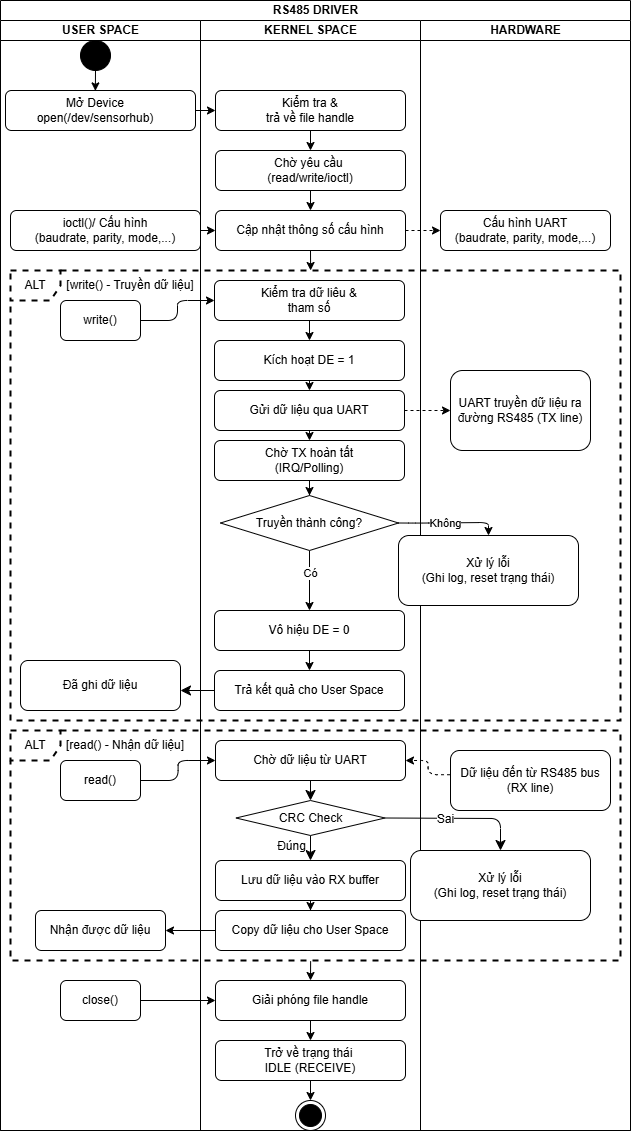
\includegraphics[width=0.8\linewidth]{image/rs485act.png}
    \caption{Activity Diagram của driver RS485}
    \label{fig:rs485_activity}
\end{figure}

Hình \ref{fig:rs485_activity} mô tả luồng hoạt động tổng quát của driver RS485 trong môi trường Linux Embedded, bao gồm sự tương tác giữa User Space, Kernel Space và phần cứng UART/RS485. Quá trình hoạt động bắt đầu khi ứng dụng ở User Space thực hiện lời gọi hệ thống \texttt{open()} để truy cập device file \texttt{/dev/sensorhub}. Khi đó, driver trong Kernel Space sẽ kiểm tra và khởi tạo file handle trước khi chuyển sang trạng thái chờ các yêu cầu xử lý như \texttt{read()}, \texttt{write()} hoặc \texttt{ioctl()}.

Đối với cơ chế cấu hình thiết bị, ứng dụng có thể sử dụng \texttt{ioctl()} để thay đổi các tham số truyền thông như baudrate, parity hoặc chế độ hoạt động UART. Driver sau đó cập nhật lại cấu hình và đồng bộ các tham số này xuống phần cứng UART thông qua Serdev Framework.

Trong quá trình truyền dữ liệu, ứng dụng sử dụng lời gọi \texttt{write()} để gửi dữ liệu xuống driver. Driver sẽ kiểm tra dữ liệu đầu vào, kích hoạt chân DE nhằm chuyển transceiver RS485 sang chế độ truyền, sau đó gửi dữ liệu qua UART. Khi quá trình truyền hoàn tất, driver chờ tín hiệu xác nhận TX hoàn thành bằng cơ chế polling hoặc interrupt. Nếu truyền thành công, driver vô hiệu hóa tín hiệu DE để quay về chế độ nhận và trả kết quả cho User Space. Ngược lại, nếu xảy ra lỗi truyền thông hoặc timeout, driver sẽ thực hiện cơ chế xử lý lỗi như ghi log và reset trạng thái hoạt động.

Đối với cơ chế nhận dữ liệu, ứng dụng sử dụng lời gọi \texttt{read()} để yêu cầu đọc dữ liệu từ thiết bị. Driver sẽ chờ dữ liệu đến từ bus RS485 thông qua UART RX line. Sau khi nhận dữ liệu, driver thực hiện kiểm tra CRC nhằm xác minh tính toàn vẹn của khung Modbus RTU. Nếu CRC hợp lệ, dữ liệu sẽ được lưu vào RX buffer và sao chép sang User Space thông qua cơ chế \texttt{copy\_to\_user()}. Trong trường hợp CRC không hợp lệ hoặc xảy ra lỗi nhận dữ liệu, driver sẽ chuyển sang nhánh xử lý lỗi nhằm đảm bảo tính ổn định của hệ thống.

Sau khi hoàn tất quá trình truyền nhận, ứng dụng gọi \texttt{close()} để giải phóng file handle. Driver khi đó sẽ giải phóng tài nguyên liên quan và đưa hệ thống trở về trạng thái chờ (\texttt{IDLE}) để tiếp tục phục vụ các yêu cầu truyền nhận tiếp theo.

\subsubsection{Driver I2C}
\noindent \textbf{Mô hình FSM của driver I2C}
Để quản lý quá trình truyền nhận dữ liệu trên bus I2C, driver được thiết kế theo mô hình máy trạng thái hữu hạn (Finite State Machine – FSM). Mô hình này giúp driver kiểm soát rõ ràng các trạng thái hoạt động trong quá trình khởi tạo, cấu hình, truyền dữ liệu và xử lý lỗi khi giao tiếp với thiết bị slave thông qua giao thức I2C.

\begin{figure}[H]
    \centering
    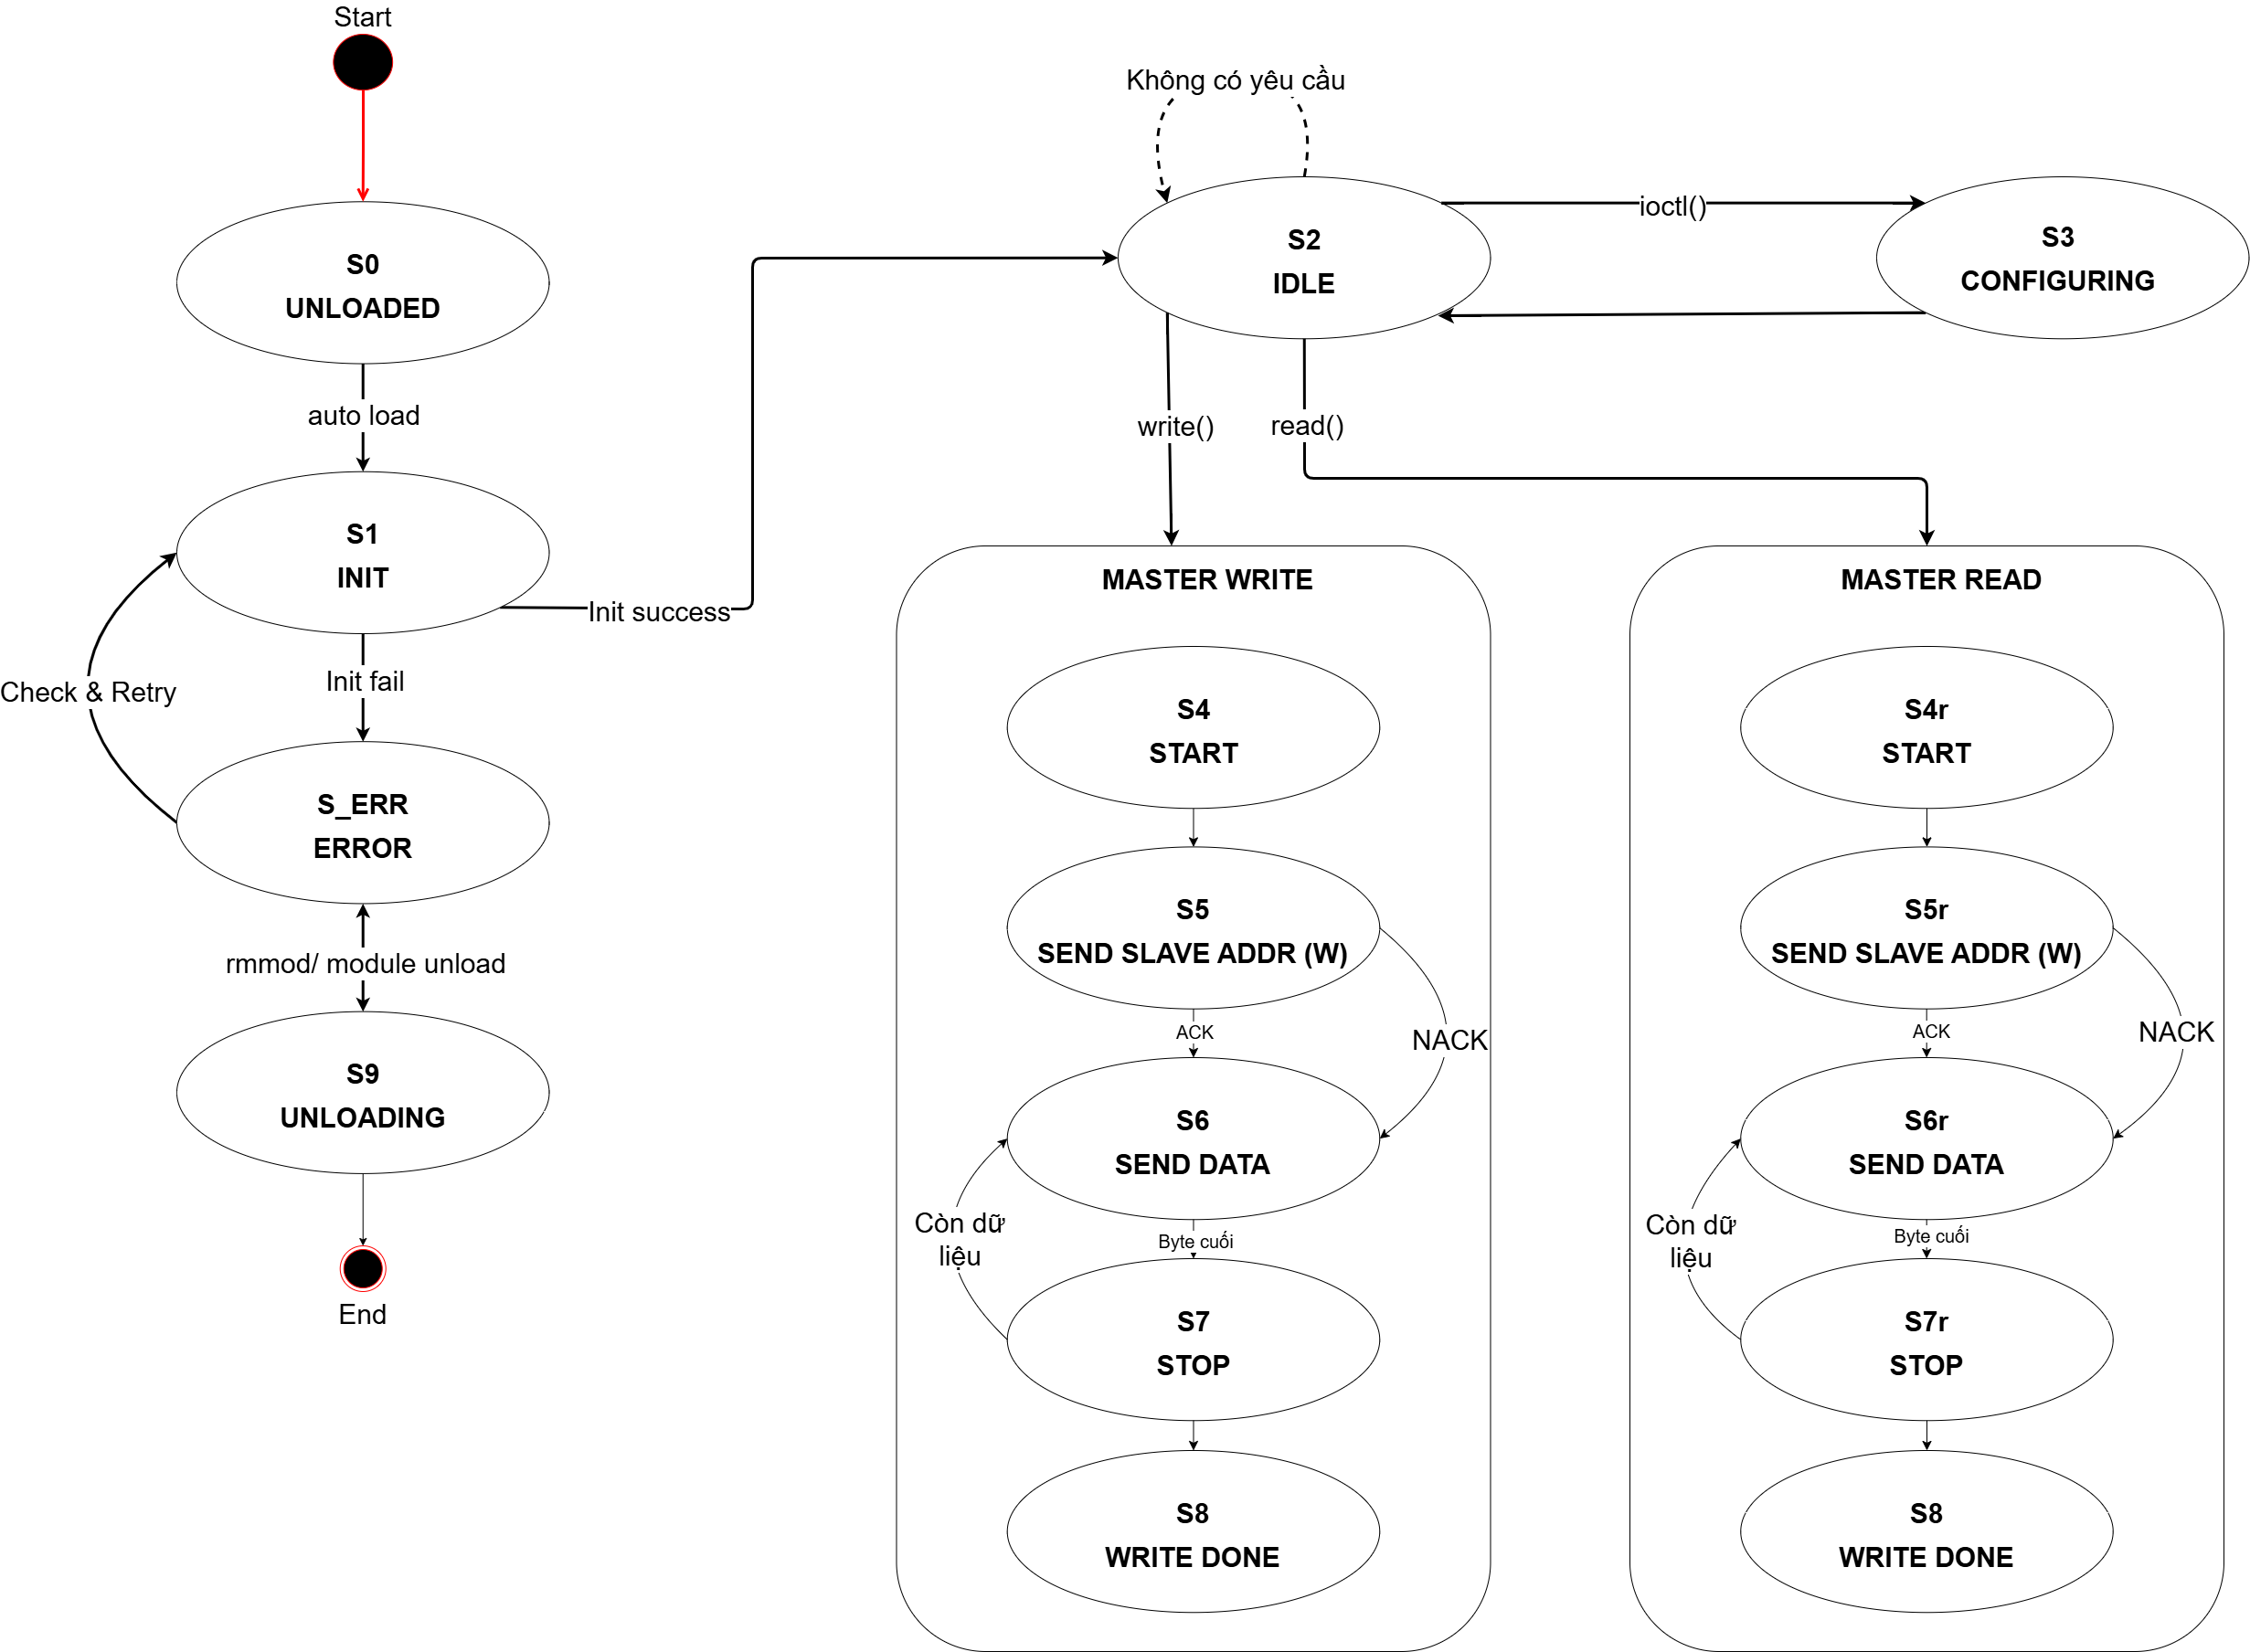
\includegraphics[width=1\linewidth]{image/i2cfsm.png}
    \caption{Máy trạng thái cho driver I2C}
    \label{fig:i2c_fsm}
\end{figure}

Quá trình hoạt động của driver bắt đầu tại trạng thái \texttt{UNLOADED}. Khi kernel module được nạp vào hệ thống thông qua cơ chế autoload hoặc lệnh \texttt{insmod}, driver chuyển sang trạng thái \texttt{INIT} để khởi tạo GPIO, cấu hình SDA/SCL và đăng ký character device với Linux Kernel. Nếu quá trình khởi tạo thành công, driver chuyển sang trạng thái \texttt{IDLE} để chờ các yêu cầu từ User Space. Ngược lại, nếu xảy ra lỗi khởi tạo, driver sẽ chuyển sang trạng thái \texttt{ERROR} để thực hiện cơ chế retry hoặc chờ unload module.

Trong trạng thái \texttt{IDLE}, driver có thể tiếp nhận các yêu cầu cấu hình thông qua lời gọi hệ thống \texttt{ioctl()}. Khi đó, driver chuyển sang trạng thái \texttt{CONFIGURING} nhằm cập nhật các tham số như địa chỉ slave, tốc độ truyền hoặc chế độ hoạt động I2C trước khi quay trở lại trạng thái chờ.

Khi ứng dụng thực hiện thao tác ghi dữ liệu thông qua \texttt{write()}, driver chuyển sang nhánh \texttt{MASTER WRITE}. Tại đây, driver lần lượt thực hiện các trạng thái bao gồm tạo tín hiệu \texttt{START}, gửi địa chỉ slave ở chế độ ghi, kiểm tra tín hiệu ACK và truyền dữ liệu lên bus I2C. Quá trình truyền tiếp tục cho đến khi byte cuối cùng được gửi thành công, sau đó driver tạo tín hiệu \texttt{STOP} và chuyển sang trạng thái \texttt{WRITE DONE}. Trong trường hợp không nhận được ACK từ slave device, driver sẽ thực hiện cơ chế xử lý lỗi hoặc retry truyền dữ liệu.

Tương tự, khi ứng dụng thực hiện thao tác đọc dữ liệu bằng \texttt{read()}, driver chuyển sang nhánh \texttt{MASTER READ}. Driver sẽ tạo tín hiệu \texttt{START}, gửi địa chỉ slave và nhận dữ liệu từ thiết bị ngoại vi thông qua bus I2C. Sau khi toàn bộ dữ liệu được nhận hoàn tất, driver tạo tín hiệu \texttt{STOP} và cập nhật dữ liệu vào buffer nội bộ trước khi trả dữ liệu về User Space.

Cuối cùng, khi kernel module bị gỡ khỏi hệ thống thông qua lệnh \texttt{rmmod}, driver chuyển sang trạng thái \texttt{UNLOADING} để giải phóng GPIO, tài nguyên kernel và character device trước khi kết thúc vòng đời hoạt động của module trong Linux Kernel.
\noindent \textbf{Activity Diagram của driver I2C}

Driver I2C được hiện thực theo mô hình Character Device trong Linux Kernel, cho phép ứng dụng ở User Space giao tiếp với thiết bị ngoại vi thông qua device file \texttt{/dev/my\_I2C\_soft}. Quá trình hoạt động của driver bao gồm các thao tác cấu hình bus, truyền dữ liệu và nhận dữ liệu thông qua cơ chế điều khiển trực tiếp các chân GPIO SDA/SCL theo chuẩn I2C software bit-banging.

Hoạt động của driver được mô tả thông qua Activity Diagram trong Hình \ref{fig:i2c_activity_diagram}.

\begin{figure}[H]
\centering
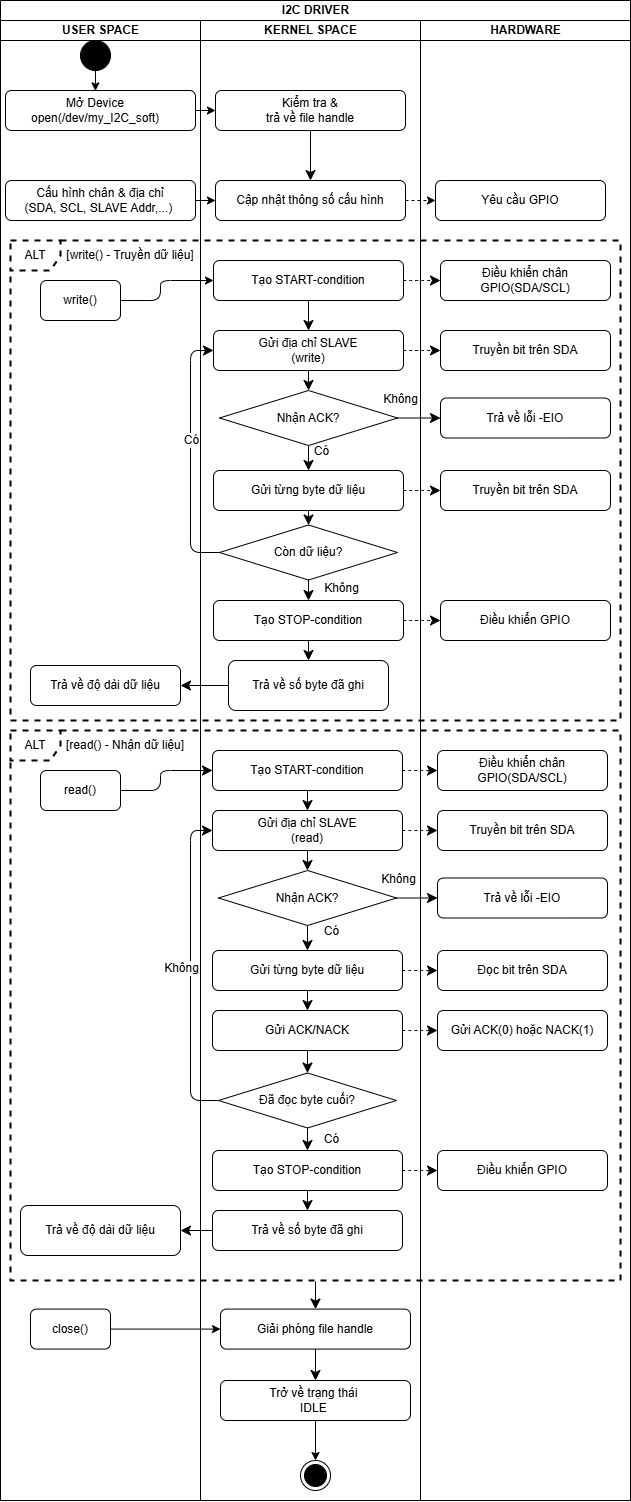
\includegraphics[width=0.65\linewidth]{image/i2cact.png}
\caption{Activity Diagram của driver I2C}
\label{fig:i2c_activity_diagram}
\end{figure}

Trong giai đoạn khởi tạo, ứng dụng User Space thực hiện lời gọi \texttt{open()} để mở device file của driver. Linux Kernel sau đó kiểm tra file handle và khởi tạo các tài nguyên cần thiết phục vụ giao tiếp I2C. Các thông số như địa chỉ slave, chân SDA/SCL và tốc độ truyền có thể được cấu hình thông qua cơ chế \texttt{ioctl()}.

Đối với quá trình truyền dữ liệu (\texttt{write()}), driver tạo điều kiện START-condition và gửi địa chỉ slave theo chế độ ghi. Sau khi nhận tín hiệu ACK từ thiết bị ngoại vi, dữ liệu sẽ được truyền tuần tự từng byte thông qua chân SDA kết hợp tín hiệu clock trên chân SCL. Nếu xảy ra lỗi ACK hoặc mất kết nối thiết bị, driver sẽ trả về lỗi \texttt{-EIO} để thông báo cho User Space. Khi hoàn tất quá trình truyền, driver tạo STOP-condition và trả về số byte đã ghi thành công.

Trong quá trình nhận dữ liệu (\texttt{read()}), driver tiếp tục tạo START-condition và gửi địa chỉ slave theo chế độ đọc. Dữ liệu từ thiết bị ngoại vi được đọc tuần tự từng byte thông qua chân SDA, đồng thời driver gửi ACK hoặc NACK tương ứng để điều khiển quá trình nhận dữ liệu. Sau khi nhận byte cuối cùng, STOP-condition được tạo ra nhằm giải phóng bus I2C trước khi dữ liệu được trả về cho User Space.

Activity Diagram cho thấy driver được tổ chức theo hướng tách biệt giữa User Space, Kernel Space và Hardware Layer. Cách tiếp cận này giúp quá trình xử lý dữ liệu trở nên rõ ràng, đồng thời hỗ trợ việc mở rộng và bảo trì driver trong các hệ thống Linux Embedded sử dụng Yocto Project.

\subsection{Thiết kế khối xử lý AI}

Mục tiêu của khối xử lý AI là xây dựng một mô hình học sâu có khả năng khai thác các đặc trưng tiềm ẩn trong dữ liệu chuỗi thời gian từ hệ thống cảm biến môi trường, từ đó đưa ra dự báo nồng độ bụi mịn PM2.5 trong tương lai với độ chính xác cao. Khối này đóng vai trò là thành phần cốt lõi của hệ thống Edge AI, cho phép thiết bị Raspberry Pi 4 thực hiện suy luận trực tiếp tại hiện trường mà không phụ thuộc vào máy chủ đám mây.
\begin{figure}[H]
    \centering
    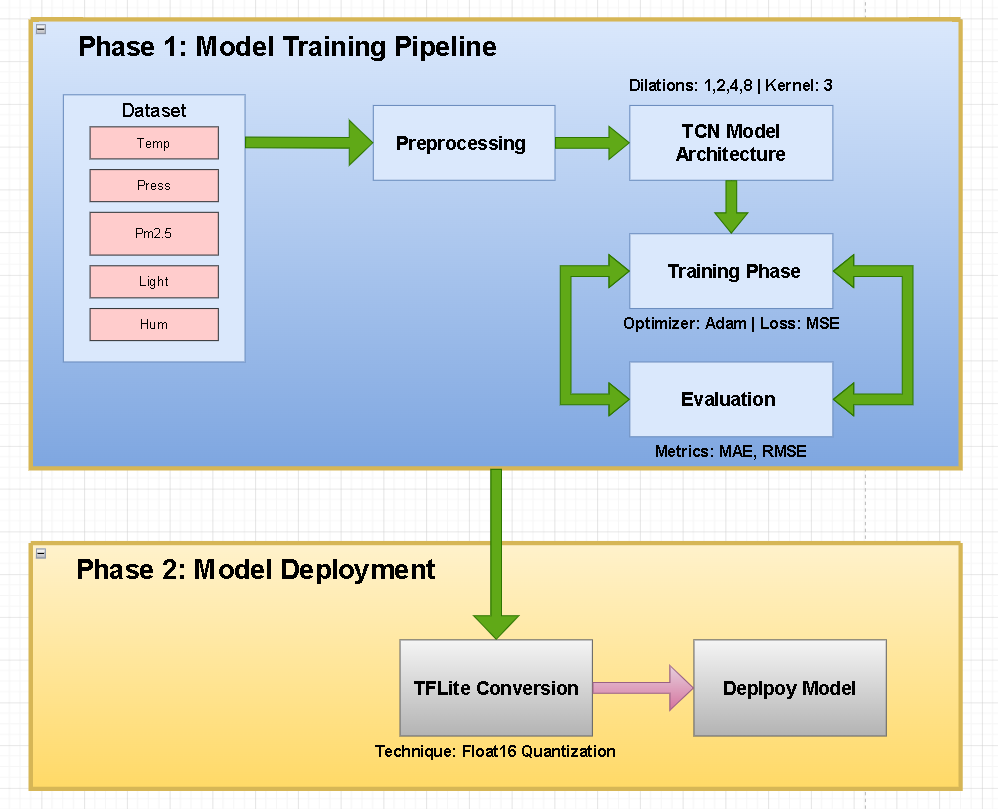
\includegraphics[width=0.8\linewidth]{image/SO_DOAI.png}
    \caption{Sơ đồ khối Module AI}
    \label{fig:placeholder}
\end{figure}
\subsubsection{Thiết kế dữ liệu đầu vào và đầu ra}

Dữ liệu môi trường thu thập được có dạng chuỗi thời gian đa biến (\textit{Multivariate Time Series}), trong đó mỗi mẫu dữ liệu bao gồm đồng thời nhiều thông số vật lý đo được tại cùng một thời điểm. Để chuyển đổi dữ liệu này thành dạng phù hợp cho mô hình học sâu, hệ thống sử dụng kỹ thuật cửa sổ trượt (\textit{Sliding Window}) nhằm xây dựng các cặp dữ liệu đầu vào -- đầu ra theo phương pháp học có giám sát.

\begin{itemize}
    \item \textbf{Vector đầu vào ($X$):}  
    Được biểu diễn dưới dạng ma trận có kích thước $(T \times F)$, trong đó:
    \begin{itemize}
        \item $T = 30$: số bước thời gian quan sát trong quá khứ.
        \item $F = 5$: số đặc trưng đầu vào, bao gồm Temperature, Humidity, Pressure, PM2.5 và Light .
    \end{itemize}

    Điều này có nghĩa là tại mỗi lần dự báo, mô hình sẽ sử dụng 30 mẫu dữ liệu gần nhất để phân tích xu hướng biến động của môi trường.

    \item \textbf{Giá trị đầu ra ($y$):}  
    Là giá trị nồng độ PM2.5 tại thời điểm $t + 15$ phút. Việc lựa chọn khoảng thời gian dự báo 15 phút giúp hệ thống có đủ thời gian để phát hiện xu hướng ô nhiễm và kích hoạt các cơ chế điều khiển phù hợp.
\end{itemize}

\subsubsection{Quy trình tiền xử lý và chuẩn hóa dữ liệu}

Dữ liệu thu thập từ các cảm biến thường có đơn vị đo và miền giá trị khác nhau. Ví dụ, nhiệt độ được đo theo độ C, áp suất theo hPa, trong khi cường độ ánh sáng có thể dao động trên dải giá trị rất lớn. Nếu đưa trực tiếp các dữ liệu này vào mô hình, các đặc trưng có biên độ lớn sẽ chi phối quá trình tối ưu hóa và làm giảm hiệu quả học của mạng nơ-ron.

Để khắc phục vấn đề này, toàn bộ dữ liệu được chuẩn hóa về khoảng $[0, 1]$ bằng phương pháp Min-Max Scaling.

\[
x' = \frac{x - x_{\min}}{x_{\max} - x_{\min}}
\]

Trong đó:

\begin{itemize}
    \item $x$: Giá trị thực tế của cảm biến.
    \item $x_{\min}$: Giá trị nhỏ nhất của đặc trưng trong tập huấn luyện.
    \item $x_{\max}$: Giá trị lớn nhất của đặc trưng trong tập huấn luyện.
\end{itemize}

Phương pháp chuẩn hóa này giúp các đặc trưng có cùng thang đo, từ đó cải thiện tốc độ hội tụ, tăng tính ổn định và nâng cao độ chính xác của mô hình.

\subsubsection{Kiến trúc mạng nơ-ron TCN (Temporal Convolutional Network)}

Mô hình được xây dựng dựa trên kiến trúc TCN, một cấu trúc mạng tích chập được thiết kế chuyên biệt cho bài toán chuỗi thời gian. So với các kiến trúc hồi tiếp như RNN hay LSTM, TCN có ưu điểm về khả năng xử lý song song, tốc độ huấn luyện nhanh và khả năng học phụ thuộc dài hạn hiệu quả.
\begin{figure}[H]
    \centering
    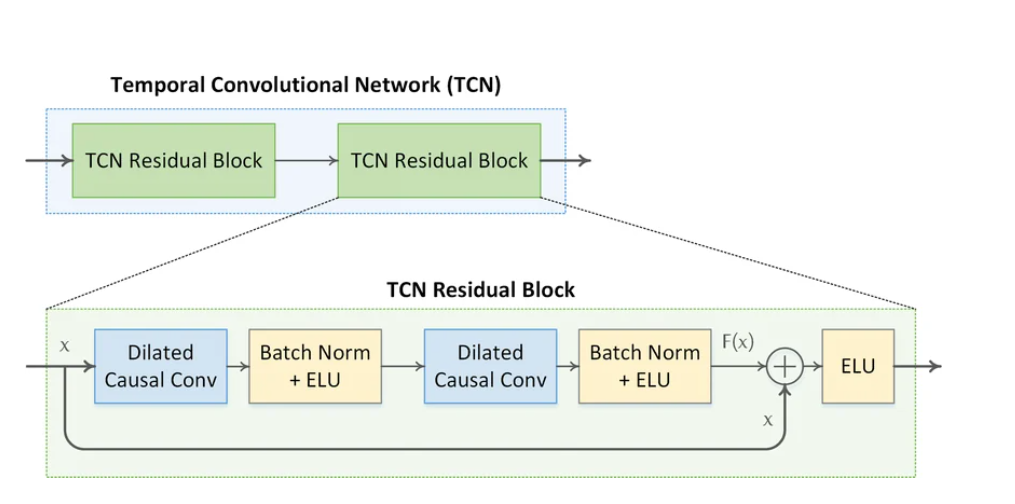
\includegraphics[width=0.8\linewidth]{image/TCN_sodo.png}
    \caption{mô hình TCN}
    \label{fig:placeholder}
\end{figure}
\textbf{Mô hình bao gồm ba thành phần cốt lõi sau.}

\paragraph{a. Tích chập nhân quả (Causal Convolution)}

Tích chập nhân quả đảm bảo rằng tại thời điểm dự báo $t$, mô hình chỉ được phép sử dụng thông tin từ quá khứ và hiện tại, tức là các phần tử $x_1, x_2, \ldots, x_t$. Cơ chế này giúp ngăn chặn hiện tượng rò rỉ thông tin từ tương lai vào quá trình học.

\paragraph{b. Tích chập giãn cách (Dilated Convolution)}

Để mở rộng trường thụ cảm mà không làm tăng đáng kể số lượng tham số, mô hình sử dụng các lớp tích chập với hệ số giãn cách $d$.

\[
(F *_d x)(s) = \sum_{i=0}^{k-1} F(i) \cdot x(s - d \cdot i)
\]

Trong đó:

\begin{itemize}
    \item $k$: Kích thước kernel tích chập, được lựa chọn bằng 3.
    \item $d$: Hệ số giãn cách.
\end{itemize}

Trong đề tài này, các hệ số giãn cách được thiết kế theo cấp số nhân:

\[
d = \{1, 2, 4, 8\}
\]

Cấu hình này giúp mô hình mở rộng trường thụ cảm theo cấp số nhân, cho phép học hiệu quả các xu hướng dài hạn của chuỗi dữ liệu.

\paragraph{c. Kết nối tắt (Residual Connections)}

Kết nối tắt giúp cải thiện quá trình lan truyền đạo hàm và hạn chế hiện tượng mất mát đạo hàm khi mạng trở nên sâu hơn.

\[
o = \text{Activation}(x + \mathcal{F}(x))
\]

Trong đó $\mathcal{F}(x)$ là hàm biến đổi phi tuyến của khối tích chập, còn $x$ là tín hiệu đầu vào được cộng trực tiếp vào đầu ra của khối.

\subsubsection{Thiết kế chiến lược huấn luyện}

Quá trình huấn luyện mô hình được thực hiện với mục tiêu tối thiểu hóa sai số giữa giá trị dự báo và giá trị thực tế.

\begin{itemize}
    \item \textbf{Hàm mất mát (Loss Function):}  
    Sai số bình phương trung bình (Mean Squared Error -- MSE) được lựa chọn do phù hợp với bài toán hồi quy.

    \[
    MSE = \frac{1}{N}\sum_{i=1}^{N}(y_i - \hat{y}_i)^2
    \]

    Trong đó $y_i$ là giá trị thực tế và $\hat{y}_i$ là giá trị dự báo của mô hình.

    \item \textbf{Thuật toán tối ưu:}  
    Adam Optimizer được sử dụng với tốc độ học (\textit{learning rate}) $\eta = 0.001$. Thuật toán này kết hợp ưu điểm của Momentum và RMSProp, giúp mô hình hội tụ nhanh và ổn định hơn so với phương pháp gradient descent truyền thống.
\end{itemize}

Ngoài ra, trong quá trình huấn luyện, tập dữ liệu được chia thành tập huấn luyện và tập kiểm thử để đánh giá khả năng tổng quát hóa của mô hình.

\subsubsection{Thiết kế quy trình tối ưu hóa Edge AI (TFLite Quantization)}

Sau khi huấn luyện hoàn tất, mô hình được chuyển đổi sang định dạng TensorFlow Lite để triển khai trên Raspberry Pi 4.

Kỹ thuật \textit{Float16 Quantization} được áp dụng để nén các trọng số từ định dạng Float32 xuống Float16. Quá trình này giúp giảm đáng kể dung lượng mô hình trong khi vẫn duy trì độ chính xác gần như tương đương với mô hình gốc.

Các lợi ích chính của quá trình tối ưu hóa bao gồm:

\begin{itemize}
    \item Giảm khoảng 50\% kích thước tệp mô hình.
    \item Tăng tốc độ suy luận trên thiết bị biên.
    \item Giảm nhu cầu sử dụng bộ nhớ RAM.
    \item Duy trì độ chính xác ở mức cao.
\end{itemize}

Nhờ quá trình tối ưu hóa này, mô hình TCN có thể hoạt động hiệu quả trên Raspberry Pi 4, đáp ứng yêu cầu xử lý thời gian thực trong hệ thống giám sát và dự báo chất lượng không khí.

\subsubsection{Mô hình FSM khối AI}
Để quản lý toàn bộ vòng đời suy luận, tối ưu hóa tài nguyên RAM và đảm bảo tính hoạt động ổn định của mô hình mạng TCN (Temporal Convolutional Network) trong không gian người dùng (User Space), khối xử lý AI được cấu trúc vận hành dựa trên một máy trạng thái hữu hạn (FSM) bao gồm các trạng thái chính sau:
\begin{figure}[H]
    \centering
    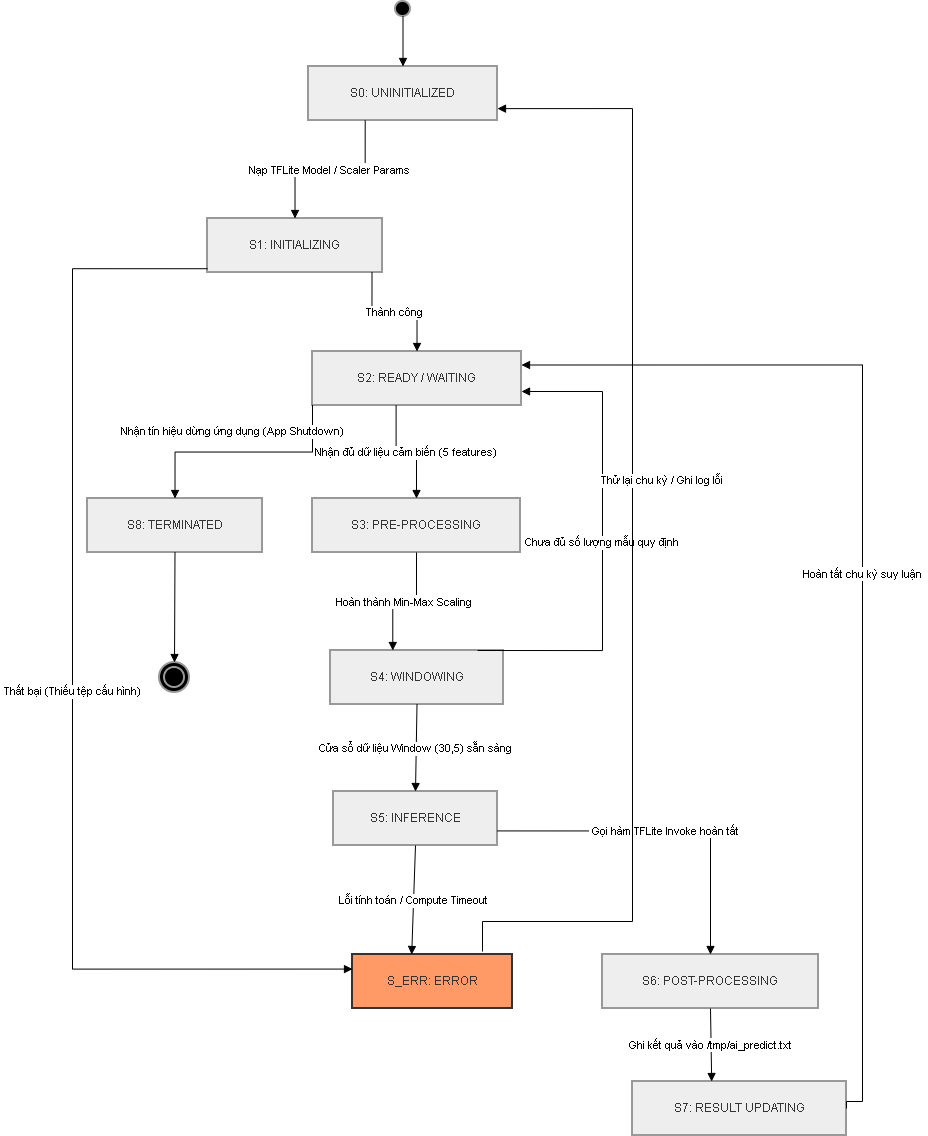
\includegraphics[width=0.7\linewidth]{image/Untitled Diagram-Page-1.drawio.png}
    \caption{Mô hình FSM khối AI}
    \label{fig:FSM_AI}
\end{figure}
\begin{itemize}
    \item S0 (UNINITIALIZED): Trạng thái khởi đầu khi tiến trình AI Engine được kích hoạt, các vùng đệm dữ liệu và mô hình chưa được nạp vào bộ nhớ.

    \item S1 (INITIALIZING): Nạp mô hình \texttt{tcn\_model\_production.tflite}, khởi tạo TFLite Interpreter và đọc các tham số chuẩn hóa từ \texttt{scaler\_params.json}.

    \item S2 (READY / WAITING): Trạng thái chờ dữ liệu cảm biến mới từ Gateway Service.

    \item S3 (PRE-PROCESSING): Thực hiện lọc trung bình trượt và chuẩn hóa 5 đặc trưng đầu vào về miền giá trị $[0,1]$.

    \item S4 (WINDOWING): Đưa dữ liệu vào hàng đợi và kiểm tra đủ 30 mẫu liên tiếp để tạo tensor đầu vào kích thước $30 \times 5$.

    \item S5 (INFERENCE): Gọi TFLite Interpreter để thực hiện suy luận với mô hình TCN.

    \item S6 (POST-PROCESSING): Thực hiện inverse scaling để chuyển kết quả dự báo về đơn vị PM2.5 gốc tại thời điểm $t+15$ phút.

    \item S7 (RESULT UPDATING): Lưu kết quả vào \texttt{/tmp/ai\_predict.txt}, giải phóng bộ đệm và quay lại trạng thái S2.

    \item S8 (TERMINATED): Giải phóng bộ nhớ và hủy TFLite Interpreter khi nhận tín hiệu dừng hệ thống.

    \item S\_ERR (ERROR): Xử lý các lỗi như lỗi nạp mô hình, dữ liệu không hợp lệ hoặc timeout, ghi log và khởi động lại tiến trình từ trạng thái S0.
\end{itemize}
\subsection{Thiết kế khối xử lý OTA}

Khối OTA được thiết kế như một thực thể quản lý vòng đời cập nhật của hệ thống, từ giai đoạn tiếp nhận gói dữ liệu đến giai đoạn tráo đổi phân vùng khởi động. Toàn bộ logic được đóng gói trong một quy trình khép kín nhằm đảm bảo tính nguyên tử (\textit{Atomicity}) và khả năng tự phục hồi (\textit{Recovery}).
\begin{figure}[H]
    \centering
    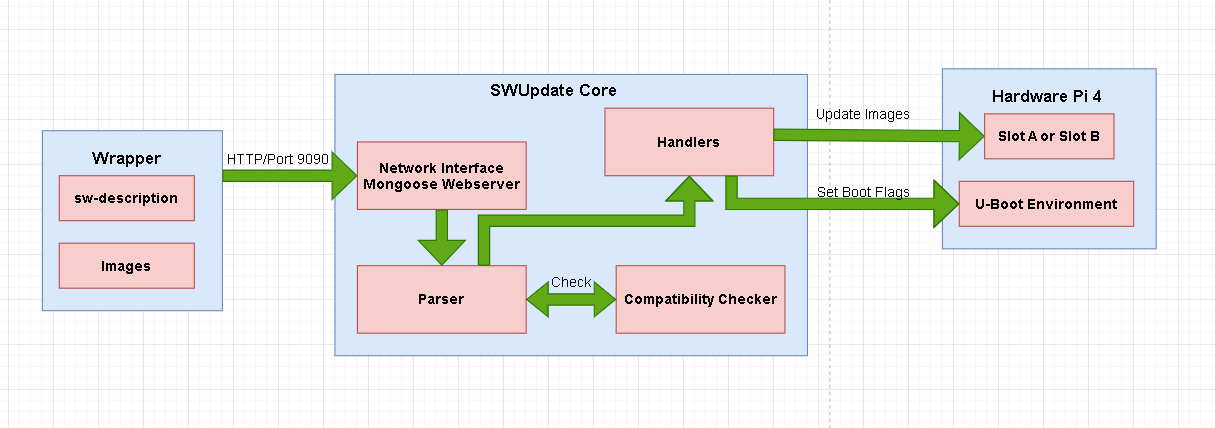
\includegraphics[width=1.0\linewidth]{image/Block_OTA.png}
    \caption{Sơ đồ khối OTA}
    \label{fig:placeholder}
\end{figure}
\subsubsection{Mô tả chi tiết các thành phần hệ thống}

\begin{itemize}
    \item \textbf{Wrapper (Gói cập nhật .swu):} Là một trình bao gói chứa đựng tệp mô tả \texttt{sw-description} và các tệp ảnh hệ thống (\textit{Images}). Thiết kế này đảm bảo tính nhất quán giữa chỉ thị cài đặt và dữ liệu thực thi.

    \item \textbf{Network Interface (Mongoose Webserver):} Được cấu hình hoạt động như một HTTP Server tại cổng 9090. Thành phần này chịu trách nhiệm tiếp nhận luồng dữ liệu (\textit{Streaming}) từ người dùng và đẩy trực tiếp vào bộ phận phân tích mà không cần lưu trữ tạm thời, giúp tối ưu hóa tài nguyên RAM cho Raspberry Pi 4.

    \item \textbf{Parser (Bộ phân tích cú pháp Libconfig):} Đóng vai trò là trung tâm điều khiển của hệ thống. Khối này giải mã các chỉ thị từ \texttt{sw-description}, xác định logic cài đặt, vị trí phân vùng đích và các ràng buộc về phần cứng.

    \item \textbf{Compatibility Checker:} Thực hiện cơ chế kiểm tra chéo giữa \textit{Hardware ID} trong gói cập nhật và thông tin phần cứng thực tế của thiết bị. Đây là chốt chặn an toàn nhằm ngăn ngừa các bản cập nhật không tương thích gây lỗi hệ thống (\textit{brick}).

    \item \textbf{Handlers (Trình thực thi):} Gồm các module chuyên biệt (Raw/Archive Handler) có nhiệm vụ giải nén và ghi trực tiếp dữ liệu vào các phân vùng vật lý. Sau khi ghi hoàn tất, Handlers sẽ thực hiện kiểm tra mã băm (\textit{Checksum}) để xác minh tính toàn vẹn của dữ liệu trên đĩa.
\end{itemize}

\subsubsection{Luồng dữ liệu và logic xử lý (Data Flow Description)}

Quy trình xử lý một bản cập nhật được thiết kế theo luồng liên kết chặt chẽ giữa các khối chức năng, mô tả như sau:

\begin{enumerate}
    \item \textbf{Giai đoạn tiếp nhận và phân tích:} Luồng dữ liệu từ tệp \texttt{.swu} đi qua Network Interface và được chuyển tiếp ngay lập tức đến Parser. Parser thực hiện bóc tách các siêu dữ liệu (\textit{Metadata}) để chuẩn bị cho các bước thẩm định tiếp theo.

    \item \textbf{Giai đoạn thẩm định và ánh xạ:} Parser gửi tín hiệu đến Compatibility Checker để xác nhận ID phần cứng. Nếu khớp, hệ thống truy vấn U-Boot Environment để xác định trạng thái của Slot A và Slot B. Dựa trên cơ chế \textit{Dual-bank}, hệ thống sẽ chọn phân vùng \textit{Passive} (đang không hoạt động) làm mục tiêu cập nhật.

    \item \textbf{Giai đoạn thực thi song song (Dual-action):} Sau khi Parser ra chỉ thị, khối Handlers thực hiện hai luồng hành động chính:
    \begin{itemize}
        \item \textbf{Update Images:} Trích xuất và ghi trực tiếp tệp \texttt{rootfs.ext4.gz} vào phân vùng đã chọn (Slot A hoặc Slot B).

        \item \textbf{Integrity Check:} Thực hiện xác minh Checksum sau khi ghi xong 100\% dữ liệu để đảm bảo không có lỗi bit xảy ra trong quá trình I/O.
    \end{itemize}

    \item \textbf{Giai đoạn xác lập (Finalization):} Chỉ khi giai đoạn thực thi thành công hoàn toàn, Handlers mới thực hiện luồng tác động cuối cùng vào U-Boot Environment thông qua lệnh Set Boot Flags (ví dụ thiết lập biến \texttt{ustate=1}). Thao tác này đánh dấu bản cập nhật đã sẵn sàng, hoàn tất tính nguyên tử của quy trình.

    \item \textbf{Tái khởi động:} Hệ thống phát lệnh khởi động lại để Bootloader thực hiện tráo đổi Slot khởi động dựa trên các cờ hiệu đã thiết lập.
\end{enumerate}

\subsubsection{Mô hình FSM khối OTA}

Nhằm đảm bảo tính an toàn, khả năng chịu lỗi cao (Fault Tolerance) và duy trì tính sẵn sàng liên tục của hệ thống theo cơ chế cập nhật Dual Partition (A/B Switching), tiến trình OTA trong không gian người dùng (User Space) được tổ chức dưới dạng máy trạng thái hữu hạn (Finite State Machine -- FSM). Mô hình này kiểm soát toàn bộ vòng đời cập nhật firmware theo cơ chế nguyên tử (Atomicity), đồng thời hỗ trợ khả năng chống hỏng hệ thống (anti-bricking).

\begin{figure}[H]
    \centering
    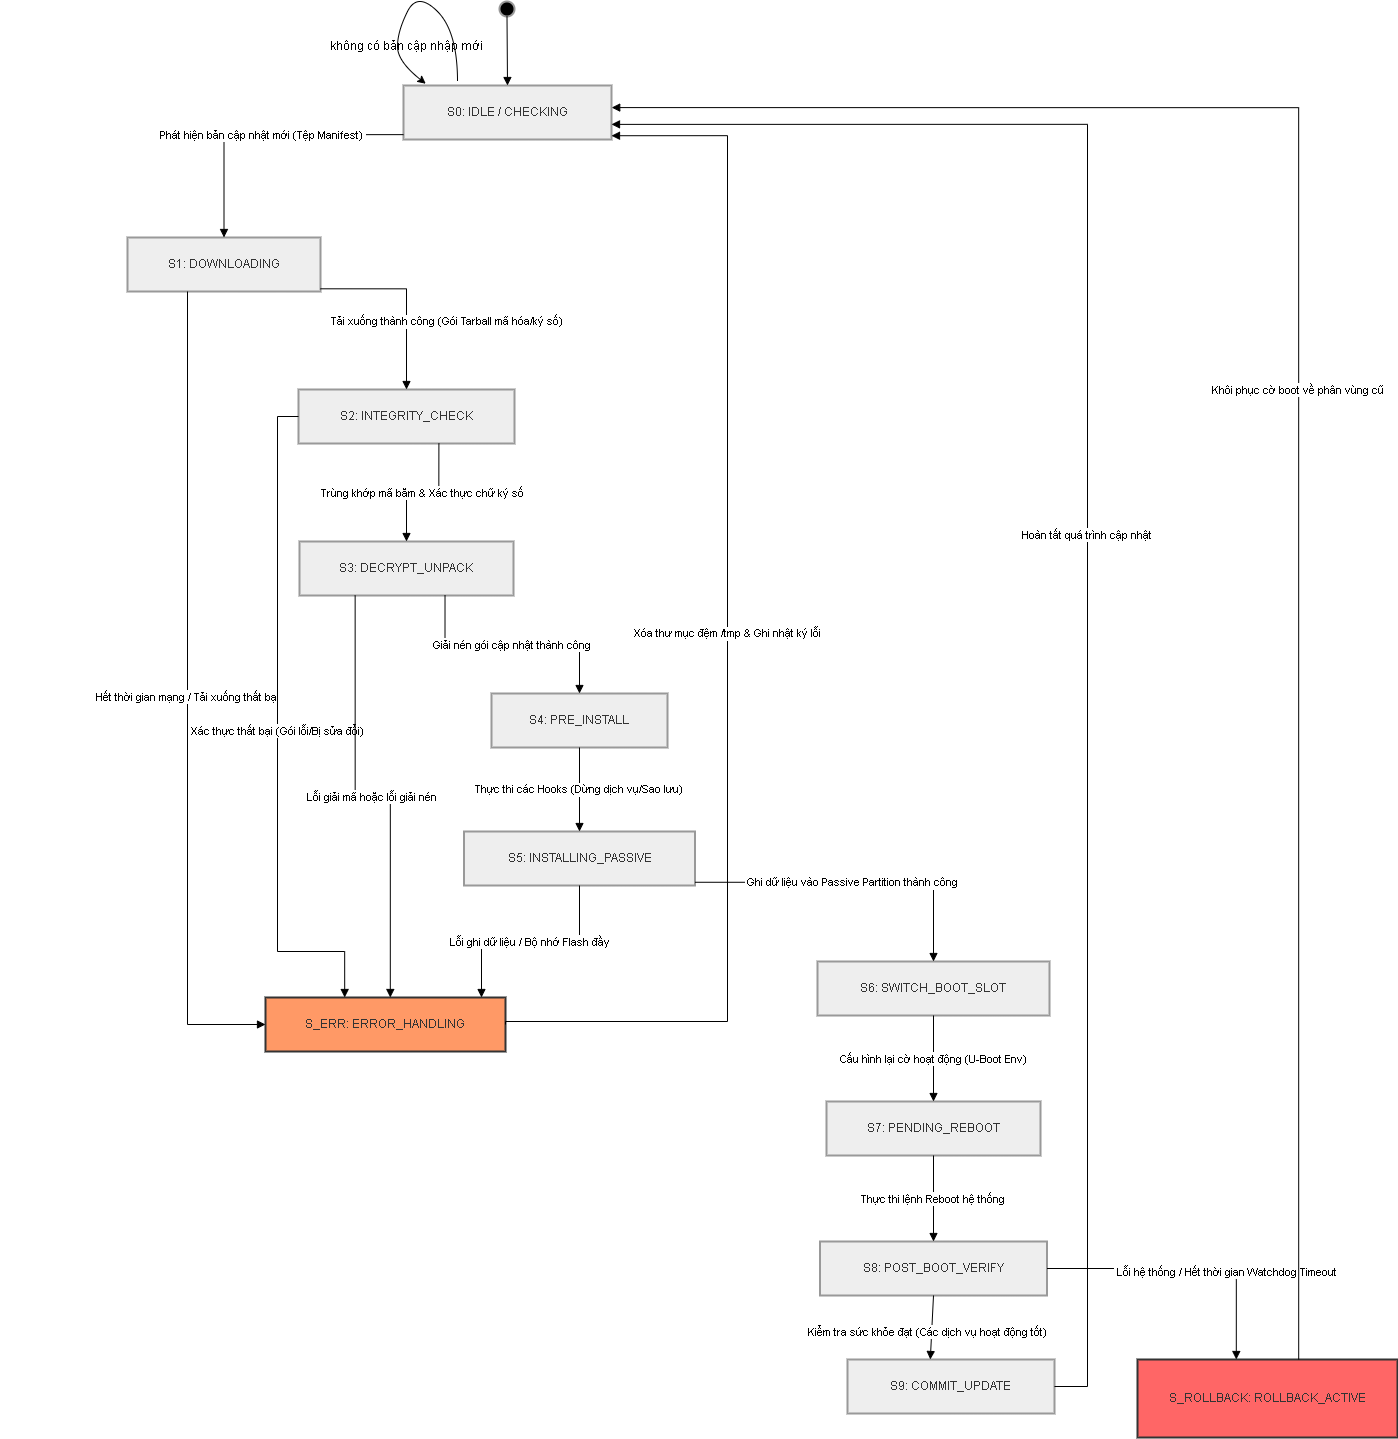
\includegraphics[width=0.7\linewidth]{image/Untitled Diagram-Page-2.drawio.png}
    \caption{Mô hình FSM khối OTA}
    \label{fig:FSM_OTA}
\end{figure}

\begin{itemize}
    \item S0 (IDLE / CHECKING): Trạng thái chờ và kiểm tra định kỳ. Gateway gửi yêu cầu HTTPS đến Deployment Server để tải tệp Manifest và so sánh phiên bản hiện tại với phiên bản mới nhất.
    \begin{itemize}
        \item Điều kiện chuyển dịch 1: Nếu không có bản cập nhật mới, hệ thống tiếp tục duy trì ở trạng thái S0.
        \item Điều kiện chuyển dịch 2: Nếu phát hiện phiên bản mới, hệ thống chuyển sang trạng thái S1.
    \end{itemize}

    \item S1 (DOWNLOADING): Trạng thái tải gói cập nhật (\texttt{.swu} hoặc \texttt{.tar.gz}) về thư mục tạm \texttt{/tmp}.
    \begin{itemize}
        \item Điều kiện chuyển dịch 1: Nếu tải xuống thành công, hệ thống chuyển sang trạng thái S2.
        \item Điều kiện chuyển dịch 2: Nếu xảy ra lỗi mạng hoặc timeout, hệ thống chuyển sang trạng thái S\_ERR.
    \end{itemize}

    \item S2 (INTEGRITY\_CHECK): Trạng thái kiểm tra mã băm SHA-256 và xác thực chữ ký số của gói cập nhật.
    \begin{itemize}
        \item Điều kiện chuyển dịch 1: Nếu mã băm trùng khớp và chữ ký hợp lệ, hệ thống chuyển sang trạng thái S3.
        \item Điều kiện chuyển dịch 2: Nếu xác thực thất bại, hệ thống chuyển sang trạng thái S\_ERR.
    \end{itemize}

    \item S3 (DECRYPT\_UNPACK): Trạng thái giải mã (nếu có) và giải nén các thành phần Kernel, DTB và RootFS.
    \begin{itemize}
        \item Điều kiện chuyển dịch 1: Nếu giải nén thành công, hệ thống chuyển sang trạng thái S4.
        \item Điều kiện chuyển dịch 2: Nếu xảy ra lỗi giải mã hoặc giải nén, hệ thống chuyển sang trạng thái S\_ERR.
    \end{itemize}

    \item S4 (PRE\_INSTALL): Trạng thái thực thi các hook tiền cài đặt như dừng dịch vụ cảm biến, AI Engine và đồng bộ dữ liệu.
    \begin{itemize}
        \item Điều kiện chuyển dịch: Sau khi hoàn tất các tác vụ chuẩn bị, hệ thống chuyển sang trạng thái S5.
    \end{itemize}

    \item S5 (INSTALLING\_PASSIVE): Trạng thái ghi firmware mới vào phân vùng không hoạt động (Passive Partition).
    \begin{itemize}
        \item Điều kiện chuyển dịch 1: Nếu ghi dữ liệu thành công, hệ thống chuyển sang trạng thái S6.
        \item Điều kiện chuyển dịch 2: Nếu xảy ra lỗi ghi dữ liệu hoặc thiếu dung lượng lưu trữ, hệ thống chuyển sang trạng thái S\_ERR.
    \end{itemize}

    \item S6 (SWITCH\_BOOT\_SLOT): Trạng thái cập nhật biến môi trường U-Boot để chọn phân vùng mới cho lần khởi động tiếp theo.
    \begin{itemize}
        \item Điều kiện chuyển dịch: Sau khi cập nhật thành công, hệ thống chuyển sang trạng thái S7.
    \end{itemize}

    \item S7 (PENDING\_REBOOT): Trạng thái thực hiện \texttt{sync} và phát lệnh khởi động lại hệ thống.
    \begin{itemize}
        \item Điều kiện chuyển dịch: Sau khi reboot, hệ thống chuyển sang trạng thái S8.
    \end{itemize}

    \item S8 (POST\_BOOT\_VERIFY): Trạng thái kiểm tra sức khỏe hệ thống sau khởi động, bao gồm các dịch vụ MQTT, cảm biến và AI Engine.
    \begin{itemize}
        \item Điều kiện chuyển dịch 1: Nếu hệ thống hoạt động ổn định, chuyển sang trạng thái S9.
        \item Điều kiện chuyển dịch 2: Nếu phát hiện lỗi hoặc timeout, chuyển sang trạng thái S\_ROLLBACK.
    \end{itemize}

    \item S9 (COMMIT\_UPDATE): Trạng thái xác nhận cập nhật bằng cách ghi cờ \texttt{boot\_successful = 1} vào U-Boot Env.
    \begin{itemize}
        \item Điều kiện chuyển dịch: Sau khi hoàn tất, hệ thống quay trở lại trạng thái S0.
    \end{itemize}

    \item S\_ROLLBACK (ROLLBACK\_ACTIVE): Trạng thái khôi phục cờ boot về phân vùng cũ ổn định và tự động khởi động lại.
    \begin{itemize}
        \item Điều kiện chuyển dịch: Sau khi rollback thành công, hệ thống ghi log lỗi và quay về trạng thái S0.
    \end{itemize}

    \item S\_ERR (ERROR\_HANDLING): Trạng thái xử lý ngoại lệ, xóa dữ liệu tạm trong \texttt{/tmp}, giải phóng tài nguyên và ghi nhật ký lỗi.
    \begin{itemize}
        \item Điều kiện chuyển dịch: Sau khi hoàn tất dọn dẹp, hệ thống quay trở lại trạng thái S0.
    \end{itemize}
\end{itemize}
    

\subsection{Thiết kế khối xử lý Tool}

Hệ thống Secure-Yocto Builder được thiết kế dựa trên mô hình kiến trúc phân lớp (\textit{Layered Architecture}), chia thành ba tầng chức năng riêng biệt nhằm đảm bảo tính module hóa, dễ dàng mở rộng và tối ưu hóa luồng xử lý dữ liệu.
\begin{figure}[H]
    \centering
    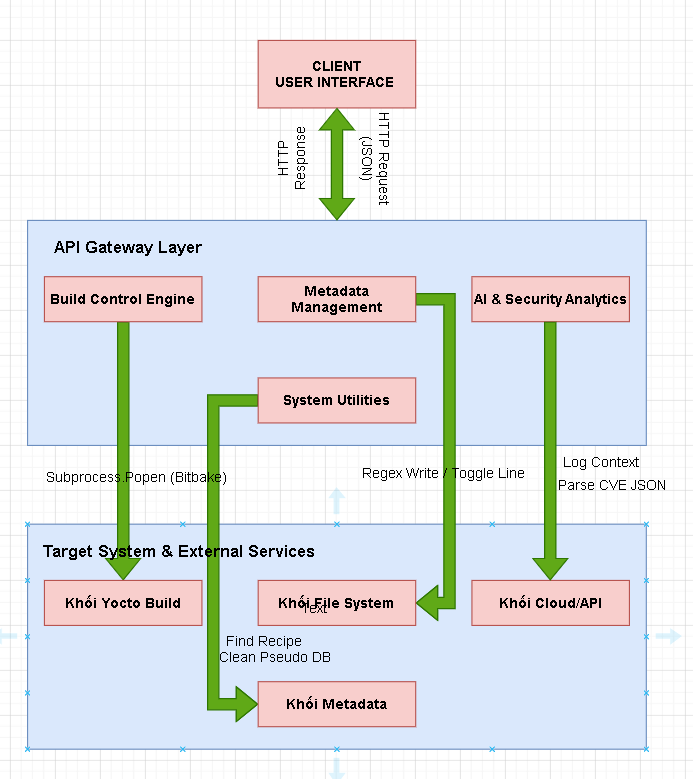
\includegraphics[width=0.70\linewidth]{image/Block_TOOl.png}
    \caption{Sơ đồ khối Tool}
    \label{fig:placeholder}
\end{figure}
\subsubsection{Lớp Giao diện Người dùng (Client User Interface)}

Lớp này đóng vai trò là bề mặt tương tác (\textit{Frontend}) của hệ thống, được xây dựng trên nền tảng Web với phong cách Terminal UI (TUI).

\begin{itemize}
    \item \textbf{Giao diện tương tác:} Cho phép người dùng tùy chỉnh các thông số cấu hình như thiết bị đích (Target), các tính năng bảo mật (SELinux, dm-verity) và nạp thư viện bổ sung.

    \item \textbf{Giao thức truyền thông:} Sử dụng phương thức gửi yêu cầu HTTP Request (định dạng JSON) tới máy chủ và nhận về các phản hồi HTTP Response để cập nhật trạng thái hệ thống theo thời gian thực.
\end{itemize}

\subsubsection{Lớp Cửa ngõ API (API Gateway Layer)}

Đây là lớp xử lý trung tâm (\textit{Backend}) sử dụng Flask Framework, đóng vai trò điều phối và thực thi các logic nghiệp vụ của ứng dụng. Lớp này bao gồm 4 module cốt lõi:

\begin{itemize}
    \item \textbf{Build Control Engine:} Điều khiển tiến trình biên dịch thông qua kỹ thuật gọi tiến trình con (\textit{subprocess}), cho phép khởi chạy lệnh \texttt{bitbake} mà không làm gián đoạn luồng xử lý chính của ứng dụng.

    \item \textbf{Metadata Management:} Chuyên trách việc thao tác dữ liệu cấu hình thông qua biểu thức chính quy (Regex), thực hiện cơ chế bật/tắt (\textit{Toggle}) các dòng mã trong file cấu hình Yocto.

    \item \textbf{AI \& Security Analytics:} Tích hợp trí tuệ nhân tạo thông qua Gemini API để phân tích ngữ cảnh lỗi (Log Context) và thực hiện phân tích cú pháp dữ liệu lỗ hổng CVE từ các tệp JSON bảo mật.

    \item \textbf{System Utilities:} Cung cấp các công cụ phụ trợ hệ thống như kiểm tra sự tồn tại của Recipe và dọn dẹp cơ sở dữ liệu cache (Pseudo DB).
\end{itemize}

\subsubsection{Lớp Hệ thống Đích và Dịch vụ Ngoại vi (Target System \& External Services)}

Đây là tầng thực thi cuối cùng, nơi chứa các tài nguyên hệ thống và các dịch vụ bên thứ ba:

\begin{itemize}
    \item \textbf{Khối Yocto Build:} Môi trường thực thi lệnh biên dịch BitBake và lưu trữ các tệp nhật ký tiến trình (Terminal Log).

    \item \textbf{Khối File System:} Lưu trữ các tệp cấu hình cốt lõi của Yocto Project như \texttt{local.conf} và \texttt{bblayers.conf}.

    \item \textbf{Khối Metadata:} Hệ thống quản lý các layer và các recipe phục vụ cho quá trình đóng gói hệ điều hành.

    \item \textbf{Khối Cloud/API:} Điểm kết nối với nền tảng điện toán đám mây để sử dụng dịch vụ AI phân tích thông minh và truy xuất dữ liệu bảo mật từ các cơ sở dữ liệu quốc gia.
\end{itemize}

\subsubsection{Mô hình FSM khối Tool }

Nhằm tự động hóa quá trình cấu hình hệ thống, quản lý tập trung các lớp metadata và tích hợp trí tuệ nhân tạo hỗ trợ phân tích lỗi biên dịch, khối Tool (Secure-Yocto Builder) được thiết kế dưới dạng máy trạng thái hữu hạn (Finite State Machine -- FSM). Mô hình này điều phối luồng dữ liệu giữa giao diện người dùng và công cụ BitBake thông qua các trạng thái xử lý sau.

\begin{figure}[H]
    \centering
    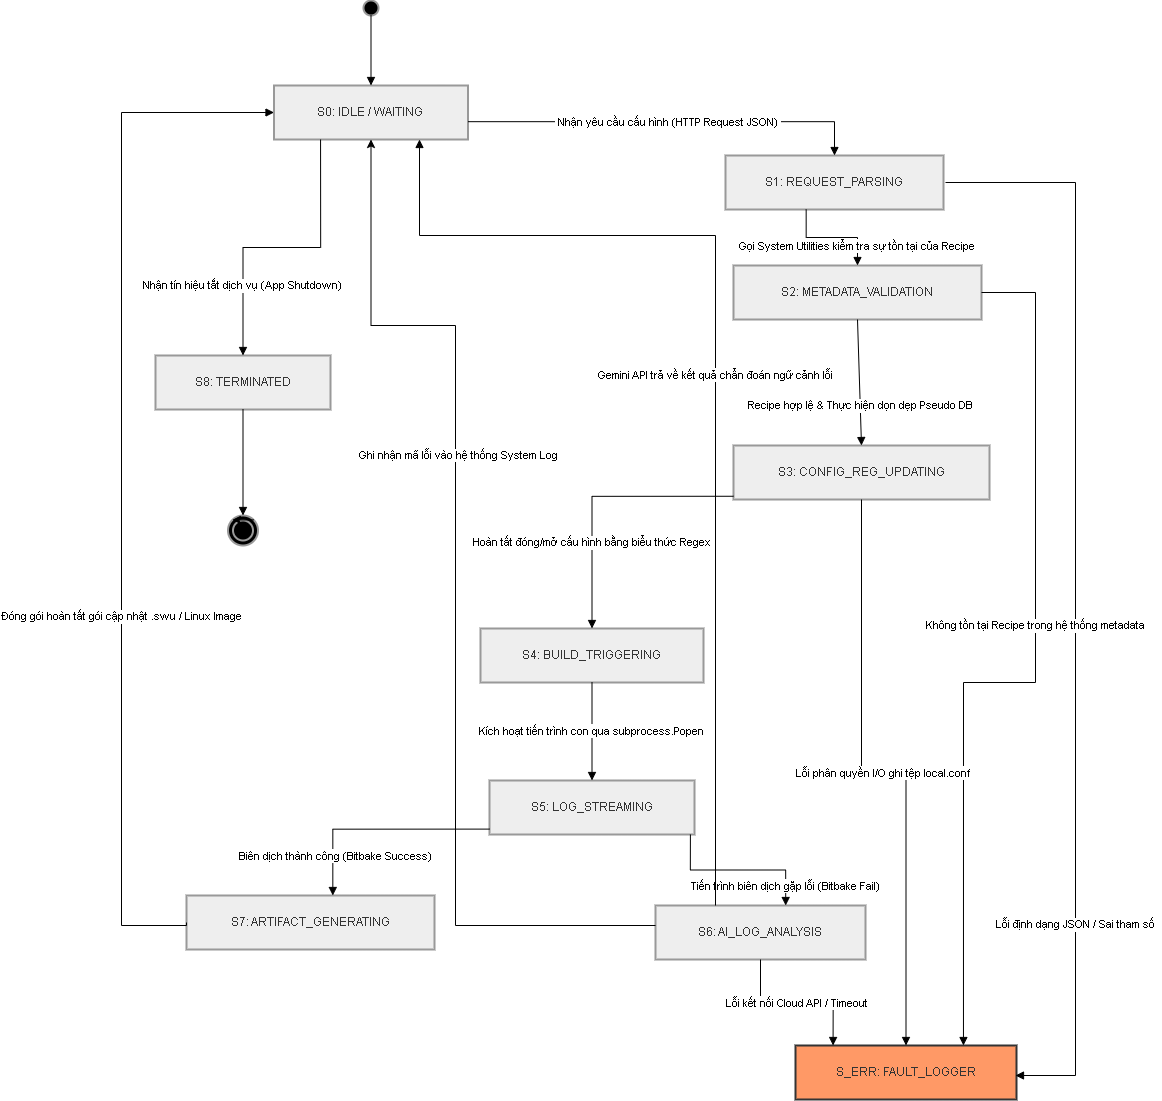
\includegraphics[width=0.70\linewidth]{image/Untitled Diagram-Page-3new.drawio.png}
    \caption{Mô hình FSM khối Tool}
    \label{fig:FSM_tool}
\end{figure}

\begin{itemize}
    \item S0 (IDLE / WAITING): Trạng thái chờ của hệ thống. Backend Flask API lắng nghe và tiếp nhận các yêu cầu cấu hình từ giao diện người dùng.

    \begin{itemize}
        \item Điều kiện chuyển dịch 1: Khi nhận được HTTP Request chứa dữ liệu JSON cấu hình, hệ thống chuyển sang trạng thái S1.
        \item Điều kiện chuyển dịch 2: Khi nhận tín hiệu tắt ứng dụng, hệ thống chuyển sang trạng thái S8.
    \end{itemize}

    \item S1 (REQUEST\_PARSING): Trạng thái phân tích cú pháp dữ liệu JSON, bao gồm thiết bị mục tiêu, các tùy chọn bảo mật và danh sách Recipe cần bổ sung.

    \begin{itemize}
        \item Điều kiện chuyển dịch 1: Nếu dữ liệu hợp lệ, hệ thống chuyển sang trạng thái S2.
        \item Điều kiện chuyển dịch 2: Nếu JSON sai định dạng hoặc thiếu tham số, hệ thống chuyển sang trạng thái S\_ERR.
    \end{itemize}

    \item S2 (METADATA\_VALIDATION): Trạng thái kiểm tra sự tồn tại của các Recipe và thực hiện dọn dẹp Pseudo DB.

    \begin{itemize}
        \item Điều kiện chuyển dịch 1: Nếu các Recipe hợp lệ, hệ thống chuyển sang trạng thái S3.
        \item Điều kiện chuyển dịch 2: Nếu Recipe không tồn tại, hệ thống chuyển sang trạng thái S\_ERR.
    \end{itemize}

    \item S3 (CONFIG\_REG\_UPDATING): Trạng thái cập nhật các tệp \texttt{local.conf} và \texttt{bblayers.conf} bằng biểu thức chính quy.

    \begin{itemize}
        \item Điều kiện chuyển dịch 1: Nếu cập nhật thành công, hệ thống chuyển sang trạng thái S4.
        \item Điều kiện chuyển dịch 2: Nếu xảy ra lỗi ghi tệp hoặc lỗi phân quyền, hệ thống chuyển sang trạng thái S\_ERR.
    \end{itemize}

    \item S4 (BUILD\_TRIGGERING): Trạng thái thiết lập môi trường và khởi chạy tiến trình biên dịch BitBake bằng \texttt{subprocess.Popen}.

    \begin{itemize}
        \item Điều kiện chuyển dịch: Sau khi tiến trình biên dịch được tạo thành công, hệ thống chuyển sang trạng thái S5.
    \end{itemize}

    \item S5 (LOG\_STREAMING): Trạng thái đọc và truyền log thời gian thực từ BitBake về giao diện người dùng.

    \begin{itemize}
        \item Điều kiện chuyển dịch 1: Nếu biên dịch thành công, hệ thống chuyển sang trạng thái S7.
        \item Điều kiện chuyển dịch 2: Nếu biên dịch thất bại, hệ thống chuyển sang trạng thái S6.
    \end{itemize}

    \item S6 (AI\_LOG\_ANALYSIS): Trạng thái gửi log lỗi đến Gemini API để phân tích nguyên nhân và đề xuất hướng khắc phục.

    \begin{itemize}
        \item Điều kiện chuyển dịch 1: Nếu nhận được kết quả phân tích, hệ thống hiển thị kết quả và quay về trạng thái S0.
        \item Điều kiện chuyển dịch 2: Nếu lỗi kết nối API hoặc timeout, hệ thống chuyển sang trạng thái S\_ERR.
    \end{itemize}

    \item S7 (ARTIFACT\_GENERATING): Trạng thái thu thập và đóng gói các tệp đầu ra như \texttt{.swu}, RootFS, Kernel Image và các artifact liên quan.

    \begin{itemize}
        \item Điều kiện chuyển dịch: Sau khi đóng gói hoàn tất, hệ thống giải phóng tài nguyên và quay về trạng thái S0.
    \end{itemize}

    \item S8 (TERMINATED): Trạng thái dừng an toàn. Hệ thống đóng Flask Backend, dừng các tiến trình con đang chạy và giải phóng tài nguyên trước khi kết thúc.

    \item S\_ERR (FAULT\_LOGGER): Trạng thái xử lý lỗi, ghi nhận nhật ký hệ thống và gửi thông báo lỗi tới giao diện người dùng.

    \begin{itemize}
        \item Điều kiện chuyển dịch: Sau khi xử lý lỗi hoàn tất, hệ thống quay trở lại trạng thái S0.
    \end{itemize}

\end{itemize}




















\section{Thiết kế dịch vụ đám mây và IoT}
\subsection{Thiết kế cơ chế truyền dữ liệu giữa Gateway và CoreIoT}

Trong hệ thống được xây dựng, Raspberry Pi 4 đóng vai trò gateway trung tâm, thực hiện chức năng thu thập dữ liệu từ các cảm biến, xử lý trạng thái hệ thống và truyền dữ liệu lên nền tảng quản lý IoT CoreIoT. Để đáp ứng yêu cầu truyền dữ liệu theo thời gian thực với mức tiêu thụ tài nguyên thấp, hệ thống sử dụng giao thức MQTT làm cơ chế giao tiếp chính giữa gateway và cloud server.

Gateway thực hiện kết nối đến MQTT Broker tại địa chỉ \texttt{App.\allowbreak coreiot.\allowbreak io} thông qua cổng \texttt{1883}. Quá trình xác thực sử dụng access token của thiết bị làm username cho phiên kết nối MQTT. Sau khi kết nối thành công, thiết bị định kỳ publish dữ liệu lên topic \texttt{v1/\allowbreak devices/\allowbreak me/\allowbreak telemetry} với chu kỳ 5 giây nhằm phục vụ việc giám sát và lưu trữ dữ liệu trên nền tảng cloud.

Dữ liệu được truyền lên hệ thống được đóng gói dưới dạng JSON nhằm đảm bảo tính linh hoạt và khả năng mở rộng trong quá trình xử lý phía server. Payload bao gồm các thông số môi trường được thu thập từ hệ thống cảm biến như nhiệt độ, độ ẩm, áp suất, cường độ ánh sáng và nồng độ bụi mịn PM2.5. Các giá trị này lần lượt được đọc từ các file trong hệ thống file của Linux như:

\begin{itemize}
    \item \texttt{/sys/class/sensorhub/hub0/temp}: dữ liệu nhiệt độ.
    \item \texttt{/sys/class/sensorhub/hub0/hum}: dữ liệu độ ẩm.
    \item \texttt{/sys/class/sensorhub/hub0/pressure}: dữ liệu áp suất môi trường.
    \item \texttt{/sys/class/sensorhub/hub0/lux}: dữ liệu cường độ ánh sáng.
    \item \texttt{/sys/class/sensorhub/hub0/pm25}: dữ liệu bụi mịn PM2.5.
\end{itemize}

Ngoài dữ liệu cảm biến thời gian thực, hệ thống còn tích hợp giá trị dự báo nồng độ PM2.5 trong 15 phút tiếp theo thông qua file tạm \texttt{/tmp/ai\_predict.txt}. Giá trị này được sử dụng nhằm hỗ trợ cơ chế cảnh báo sớm và nâng cao khả năng giám sát môi trường trong hệ thống kho thông minh.

Bên cạnh dữ liệu cảm biến, payload còn chứa các trường bổ trợ như mã thiết bị (\texttt{node}), chế độ hoạt động (\texttt{mode}) và timestamp thời gian thực nhằm hỗ trợ đồng bộ và lưu trữ dữ liệu trên nền tảng cloud. Trước khi gửi lên MQTT Broker, gateway thực hiện tiền xử lý dữ liệu để chuẩn hóa các giá trị cảm biến, trong đó nhiệt độ được chia cho 10 và áp suất được chia cho 100 để đưa về đơn vị thực tế.

Sau quá trình tiền xử lý, gateway tiến hành đánh giá trạng thái hoạt động của hệ thống dựa trên các ngưỡng cảnh báo đã được thiết lập. Nếu nhiệt độ vượt quá 45\textdegree C hoặc giá trị dự báo PM2.5 lớn hơn 100, hệ thống sẽ chuyển sang trạng thái \texttt{EMERGENCY\_FIRE} và kích hoạt quạt làm mát ở mức cao nhất nhằm đảm bảo an toàn cho môi trường vận hành.

\begin{table}[H]
\centering
\begin{tabular}{|c|c|c|}
\hline
\textbf{Điều kiện} & \textbf{Trạng thái hệ thống} & \textbf{Mức quạt} \\ \hline
Nhiệt độ $<$ 30\textdegree C & NORMAL & LOW \\ \hline
30\textdegree C $\leq$ Nhiệt độ $<$ 40\textdegree C & WARNING & MEDIUM \\ \hline
Nhiệt độ $\geq$ 40\textdegree C & CRITICAL & HIGH \\ \hline
Nhiệt độ $>$ 45\textdegree C hoặc PM2.5 dự báo $>$ 100 & EMERGENCY\_FIRE & HIGH \\ \hline
\end{tabular}
\caption{Cơ chế xác định trạng thái hệ thống}
\label{tab:system_state_logic}
\end{table}

Bên cạnh cơ chế điều khiển theo ngưỡng nhiệt độ, hệ thống còn triển khai cơ chế giám sát trạng thái kéo dài nhằm phát hiện các tình huống bất thường trong quá trình vận hành. Nếu quạt duy trì ở mức \texttt{HIGH} liên tục trong hơn 30 giây, gateway sẽ chuyển hệ thống sang trạng thái \texttt{EMERGENCY\_SYSTEM}. Cơ chế này giúp nâng cao khả năng giám sát và tăng mức độ an toàn cho hệ thống trong môi trường thực tế.

Song song với quá trình điều khiển quạt, relay cũng được điều khiển tự động dựa trên nhiệt độ môi trường. Relay sẽ được kích hoạt khi nhiệt độ vượt quá 25\textdegree C và tự động tắt khi nhiệt độ giảm xuống dưới ngưỡng quy định.

Sau khi hoàn tất quá trình xử lý và đánh giá trạng thái, gateway tiến hành tổng hợp toàn bộ dữ liệu cảm biến và trạng thái hệ thống thành một payload hoàn chỉnh trước khi gửi lên nền tảng CoreIoT thông qua giao thức MQTT. Payload được xây dựng dưới dạng JSON nhằm đảm bảo khả năng mở rộng và dễ dàng tích hợp với hệ thống backend.

Cấu trúc dữ liệu được gửi lên hệ thống được mô tả trong Bảng \ref{tab:api_payload}.

\begin{table}[H]
\centering
\begin{tabular}{|c|l|l|}
\hline
\textbf{Trường dữ liệu} & \textbf{Ý nghĩa} & \textbf{Ví dụ} \\ \hline
\texttt{temperature} & Nhiệt độ môi trường & 32.5 \\ \hline
\texttt{humidity} & Độ ẩm môi trường & 75 \\ \hline
\texttt{light\_intensity} & Cường độ ánh sáng & 420 \\ \hline
\texttt{pm25} & Nồng độ bụi mịn PM2.5 & 18 \\ \hline
\texttt{stat} & Trạng thái hệ thống & WARNING \\ \hline
\texttt{node} & Mã thiết bị gateway & ESP\_01 \\ \hline
\texttt{mode} & Chế độ hoạt động & day \\ \hline
\texttt{timestamp} & Thời gian gửi dữ liệu & 1715259000 \\ \hline
\end{tabular}
\caption{Cấu trúc payload dữ liệu gửi lên CoreIoT}
\label{tab:api_payload}
\end{table}

Từ cấu trúc trên, payload JSON được gửi lên MQTT Broker có dạng như sau:

\begin{verbatim}
{
    "temperature": 32.5,
    "humidity": 75,
    "light_intensity": 420,
    "pm25": 18,
    "stat": "WARNING",
    "node": "ESP_01",
    "mode": "day",
    "timestamp": "1715259000"
}
\end{verbatim}

\subsection{Thiết kế Rule Chain xử lý dữ liệu IoT}
Nhóm đã nghiên cứu và hiện thực cơ chế Rule Chain nhằm xử lý telemetry và điều khiển thiết bị IoT theo hướng tự động hóa. Rule Chain được triển khai trên cloud server và đóng vai trò như một pipeline xử lý dữ liệu trung tâm, cho phép tiếp nhận telemetry từ các local rule chain trên thiết bị Linux nhúng, sau đó phân tích dữ liệu, thực hiện điều khiển và phát sinh cảnh báo tương ứng. 

Các trường dữ liệu chính rule chain xử lí logic:

\begin{verbatim}
    {
    "stat": "WARNING",
    "node": "ESP_01",
    "mode": "day"
    }
\end{verbatim}  

Trong đó, trường \texttt{stat} biểu diễn trạng thái hoạt động hoặc mức độ cảnh báo của thiết bị, trường \texttt{node} dùng để định danh thiết bị gửi dữ liệu và trường \texttt{mode} biểu diễn chế độ hoạt động hiện tại của hệ thống như chế độ ngày hoặc đêm. Các telemetry này được local rule chain xử lý sơ bộ trước khi gửi lên cloud để giảm tải cho hệ thống trung tâm và tối ưu khả năng phản hồi.

Sau khi nhận telemetry, Rule Chain trên cloud sẽ sử dụng các script node để kiểm tra giá trị của từng trường dữ liệu và quyết định hướng xử lý tương ứng. Ví dụ, nếu trường \texttt{mode} có giá trị \texttt{day}, hệ thống sẽ kích hoạt các rule dành cho chế độ hoạt động ban ngày. Tương tự, khi trường \texttt{stat} mang giá trị \texttt{WARNING} hoặc \texttt{CRITICAL}, Rule Chain sẽ chuyển dữ liệu đến các node alarm để tạo cảnh báo trên Dashboard giám sát. Việc xử lý dựa trên telemetry giúp hệ thống có khả năng phản ứng tự động theo trạng thái thực tế của thiết bị.

Bên cạnh chức năng xử lý telemetry, nhóm còn tích hợp cơ chế RPC (Remote Procedure Call) nhằm hỗ trợ điều khiển thiết bị từ xa thông qua cloud server. Khi người dùng thao tác trên Dashboard, Rule Chain sẽ tạo RPC request và gửi trực tiếp đến node tương ứng dựa trên giá trị \texttt{node} trong telemetry. Thiết bị sau khi nhận RPC sẽ thực thi các tác vụ như bật hoặc tắt thiết bị, thay đổi chế độ hoạt động hoặc cập nhật trạng thái hệ thống, sau đó gửi phản hồi ngược về cloud để cập nhật trạng thái theo thời gian thực.
